\documentclass[]{book}
\usepackage{lmodern}
\usepackage{amssymb,amsmath}
\usepackage{ifxetex,ifluatex}
\usepackage{fixltx2e} % provides \textsubscript
\ifnum 0\ifxetex 1\fi\ifluatex 1\fi=0 % if pdftex
  \usepackage[T1]{fontenc}
  \usepackage[utf8]{inputenc}
\else % if luatex or xelatex
  \ifxetex
    \usepackage{mathspec}
  \else
    \usepackage{fontspec}
  \fi
  \defaultfontfeatures{Ligatures=TeX,Scale=MatchLowercase}
\fi
% use upquote if available, for straight quotes in verbatim environments
\IfFileExists{upquote.sty}{\usepackage{upquote}}{}
% use microtype if available
\IfFileExists{microtype.sty}{%
\usepackage{microtype}
\UseMicrotypeSet[protrusion]{basicmath} % disable protrusion for tt fonts
}{}
\usepackage[margin=1in]{geometry}
\usepackage{hyperref}
\hypersetup{unicode=true,
            pdftitle={Angewandte Statistische Methoden in den Nutztierwissenschaften},
            pdfauthor={Peter von Rohr},
            pdfborder={0 0 0},
            breaklinks=true}
\urlstyle{same}  % don't use monospace font for urls
\usepackage{natbib}
\bibliographystyle{apalike}
\usepackage{color}
\usepackage{fancyvrb}
\newcommand{\VerbBar}{|}
\newcommand{\VERB}{\Verb[commandchars=\\\{\}]}
\DefineVerbatimEnvironment{Highlighting}{Verbatim}{commandchars=\\\{\}}
% Add ',fontsize=\small' for more characters per line
\usepackage{framed}
\definecolor{shadecolor}{RGB}{248,248,248}
\newenvironment{Shaded}{\begin{snugshade}}{\end{snugshade}}
\newcommand{\KeywordTok}[1]{\textcolor[rgb]{0.13,0.29,0.53}{\textbf{{#1}}}}
\newcommand{\DataTypeTok}[1]{\textcolor[rgb]{0.13,0.29,0.53}{{#1}}}
\newcommand{\DecValTok}[1]{\textcolor[rgb]{0.00,0.00,0.81}{{#1}}}
\newcommand{\BaseNTok}[1]{\textcolor[rgb]{0.00,0.00,0.81}{{#1}}}
\newcommand{\FloatTok}[1]{\textcolor[rgb]{0.00,0.00,0.81}{{#1}}}
\newcommand{\ConstantTok}[1]{\textcolor[rgb]{0.00,0.00,0.00}{{#1}}}
\newcommand{\CharTok}[1]{\textcolor[rgb]{0.31,0.60,0.02}{{#1}}}
\newcommand{\SpecialCharTok}[1]{\textcolor[rgb]{0.00,0.00,0.00}{{#1}}}
\newcommand{\StringTok}[1]{\textcolor[rgb]{0.31,0.60,0.02}{{#1}}}
\newcommand{\VerbatimStringTok}[1]{\textcolor[rgb]{0.31,0.60,0.02}{{#1}}}
\newcommand{\SpecialStringTok}[1]{\textcolor[rgb]{0.31,0.60,0.02}{{#1}}}
\newcommand{\ImportTok}[1]{{#1}}
\newcommand{\CommentTok}[1]{\textcolor[rgb]{0.56,0.35,0.01}{\textit{{#1}}}}
\newcommand{\DocumentationTok}[1]{\textcolor[rgb]{0.56,0.35,0.01}{\textbf{\textit{{#1}}}}}
\newcommand{\AnnotationTok}[1]{\textcolor[rgb]{0.56,0.35,0.01}{\textbf{\textit{{#1}}}}}
\newcommand{\CommentVarTok}[1]{\textcolor[rgb]{0.56,0.35,0.01}{\textbf{\textit{{#1}}}}}
\newcommand{\OtherTok}[1]{\textcolor[rgb]{0.56,0.35,0.01}{{#1}}}
\newcommand{\FunctionTok}[1]{\textcolor[rgb]{0.00,0.00,0.00}{{#1}}}
\newcommand{\VariableTok}[1]{\textcolor[rgb]{0.00,0.00,0.00}{{#1}}}
\newcommand{\ControlFlowTok}[1]{\textcolor[rgb]{0.13,0.29,0.53}{\textbf{{#1}}}}
\newcommand{\OperatorTok}[1]{\textcolor[rgb]{0.81,0.36,0.00}{\textbf{{#1}}}}
\newcommand{\BuiltInTok}[1]{{#1}}
\newcommand{\ExtensionTok}[1]{{#1}}
\newcommand{\PreprocessorTok}[1]{\textcolor[rgb]{0.56,0.35,0.01}{\textit{{#1}}}}
\newcommand{\AttributeTok}[1]{\textcolor[rgb]{0.77,0.63,0.00}{{#1}}}
\newcommand{\RegionMarkerTok}[1]{{#1}}
\newcommand{\InformationTok}[1]{\textcolor[rgb]{0.56,0.35,0.01}{\textbf{\textit{{#1}}}}}
\newcommand{\WarningTok}[1]{\textcolor[rgb]{0.56,0.35,0.01}{\textbf{\textit{{#1}}}}}
\newcommand{\AlertTok}[1]{\textcolor[rgb]{0.94,0.16,0.16}{{#1}}}
\newcommand{\ErrorTok}[1]{\textcolor[rgb]{0.64,0.00,0.00}{\textbf{{#1}}}}
\newcommand{\NormalTok}[1]{{#1}}
\usepackage{longtable,booktabs}
\usepackage{graphicx,grffile}
\makeatletter
\def\maxwidth{\ifdim\Gin@nat@width>\linewidth\linewidth\else\Gin@nat@width\fi}
\def\maxheight{\ifdim\Gin@nat@height>\textheight\textheight\else\Gin@nat@height\fi}
\makeatother
% Scale images if necessary, so that they will not overflow the page
% margins by default, and it is still possible to overwrite the defaults
% using explicit options in \includegraphics[width, height, ...]{}
\setkeys{Gin}{width=\maxwidth,height=\maxheight,keepaspectratio}
\IfFileExists{parskip.sty}{%
\usepackage{parskip}
}{% else
\setlength{\parindent}{0pt}
\setlength{\parskip}{6pt plus 2pt minus 1pt}
}
\setlength{\emergencystretch}{3em}  % prevent overfull lines
\providecommand{\tightlist}{%
  \setlength{\itemsep}{0pt}\setlength{\parskip}{0pt}}
\setcounter{secnumdepth}{5}
% Redefines (sub)paragraphs to behave more like sections
\ifx\paragraph\undefined\else
\let\oldparagraph\paragraph
\renewcommand{\paragraph}[1]{\oldparagraph{#1}\mbox{}}
\fi
\ifx\subparagraph\undefined\else
\let\oldsubparagraph\subparagraph
\renewcommand{\subparagraph}[1]{\oldsubparagraph{#1}\mbox{}}
\fi

%%% Use protect on footnotes to avoid problems with footnotes in titles
\let\rmarkdownfootnote\footnote%
\def\footnote{\protect\rmarkdownfootnote}

%%% Change title format to be more compact
\usepackage{titling}

% Create subtitle command for use in maketitle
\newcommand{\subtitle}[1]{
  \posttitle{
    \begin{center}\large#1\end{center}
    }
}

\setlength{\droptitle}{-2em}
  \title{Angewandte Statistische Methoden in den Nutztierwissenschaften}
  \pretitle{\vspace{\droptitle}\centering\huge}
  \posttitle{\par}
  \author{Peter von Rohr}
  \preauthor{\centering\large\emph}
  \postauthor{\par}
  \predate{\centering\large\emph}
  \postdate{\par}
  \date{2017-03-26}

\usepackage{booktabs}
\usepackage{amsthm}
\makeatletter
\def\thm@space@setup{%
  \thm@preskip=8pt plus 2pt minus 4pt
  \thm@postskip=\thm@preskip
}
\makeatother

\begin{document}
\maketitle

{
\setcounter{tocdepth}{1}
\tableofcontents
}
\chapter*{Vorwort}\label{vorwort}
\addcontentsline{toc}{chapter}{Vorwort}

Dieses Dokument umfasst die kompletten Unterlagen zur Vorlesung
\textbf{Angewandte Statistische Methoden in den Nutztierwissenschaften}.
Der Titel dieser Vorlesung ist sehr allgemein gehalten. Dies würde es
erlauben einen grosszügigen Überblick über eine breite Palette an
statistischen Methoden, welche in den Nutztierwissenschaften eingesetzt
werden, zu geben.

Wir schlagen an dieser Stelle aber einen anderen Weg ein, und
fokussieren uns auf die statistischen Methoden in der genomischen
Selektion. Nur diese bewusste Wahl eines spezifischen Gebietes
ermöglicht es uns, den behandelten Stoff angemessen zu vertiefen. Im
anschliessenden Unterabschnitt wollen wir die hier getroffene
Entscheidung der Fokusierung auf die genomische Selektion motivieren.
Dabei wird klar, dass wir mit der Wahl des Themas der multiplen linearen
Regression als Ausgangspunkt auch eine Leserschaft ansprechen, welche
nicht primär an der Tierzucht interessiert ist.

\section*{Motivation}\label{motivation}
\addcontentsline{toc}{section}{Motivation}

Vom Standpunkt der statistischen Modellierung, ist das einfache lineare
Modell mit fixen Effektstufen für den Einsatz in der genomischen
Selektion ausreichend. Diese Art von Modellen werden auch als
Regressionsmodelle bezeichnet. Die Problematik entsteht erst bei der
Technik, welche wir für die Schätzung der unbekannten Parameter
verwenden können. In der klassischen Regressionsanalyse ist die Methode
der kleinsten Quadrate (Least Squares) die Methode der Wahl. Least
Squares können wir aber für die genomische Selektion nicht verwenden, da
die Anzahl unbekannter Parameter (\(p\)) grösser ist als die Anzahl
Beobachtungen (\(n\)).

Mit der steigenden Grösse und Komplexität von aktuellen Datensätzen
tritt das soeben beschriebene Problem nicht nur in der Tierzucht auf,
sondern es gibt eine breite Palette von Anwendungen. In der Vorlesung
beschrieben wir diese Problematik am Beispiel der genomischen Selektion
und es werden alternative Techniken zur Schätzung von Parametern
vorgeschlagen. Da die Methode der multiplen Regressionsanalyse in
früheren Vorlesungen behandelt wurde, bietet diese ein idealer
Ausgangspunkt für den in dieser Veranstaltung präsentierten Stoffinhalt.

\section*{Einordnung}\label{einordnung}
\addcontentsline{toc}{section}{Einordnung}

Die Vorlesung \textbf{Angewandte Statistische Methoden in den
Nutztierwissenschaften} ist eine halb-semestrige Veranstaltung und wird
im Masterstudiengang Agrarwissenschaften der ETH Zürich angeboten.

\section*{Lernziele}\label{lernziele}
\addcontentsline{toc}{section}{Lernziele}

Für die Verwendung des hier präsentierten Stoffs schlagen wir die
folgenden Lernziele vor.

Die Studierenden \ldots{}

\begin{itemize}
\tightlist
\item
  kennen die Eigenschaften der multiplen linearen Regression und
\item
  können einfache Datensätze mithilfe der Regressionsmethode analysieren
\item
  wissen wieso multiple lineare Regressionen bei der genomischen
  Selektion nicht brauchbar ist
\item
  kennen die in der genomischen Selektion verwendeten statistischen
  Verfahren, wie

  \begin{itemize}
  \tightlist
  \item
    BLUP-basierte Verfahren,
  \item
    Bayes'sche Verfahren und
  \item
    die LASSO Methode
  \end{itemize}
\item
  können einfache Übungsbeispiele mit der Statistiksoftware R
  erfolgreich bearbeiten.
\end{itemize}

\chapter{Einführung}\label{intro}

Den in dieser Vorlesung präsentierte Stoff kann aus mehreren
Gesichtspunkten betrachtet werden. Aus Sicht der Tierzucht behandeln wir
die statistischen Methoden, welche in der \textbf{genomischen Selektion}
angewendet werden. Für Statistiker stellen wir verschiedene Methoden der
Regularisierung in hoch-parametrischen Modellen vor. In der sehr
populären Disziplin des \textbf{Machine Learnings} wird das hier
besprochene Problem als die Selektion von relevanten Features im Kontext
des Supervised Learnings dargestellt.

\section{Beschreibung des Problems}\label{problem}

Alle die soeben genannten Formulierungen beschreiben das gleiche
Problem. Wir gehen von einem Datensatz aus, welcher aus Beobachtungen
besteht. Jede Beobachtung ist charakterisiert durch sehr viele
unabhängige Grössen. Die Gewichtung der zu einer Beobachtung gehörenden
Grössen wird über unbekannte Parameter erreicht.

Als Beispiel für einen solchen Datensatz können wir eine Population mit
SNP-typisierten Tieren betrachten. Das Typisierrungsergebnis für ein
bestimmtes Tier enthält die Genotypen an den Genorten, welche bei der
Typisierung untersucht werden. Die einzelnen Genorte werden als
sogenannte Single Nucleotide Polymorphisms (SNP) bezeichnet. In
Abhängigkeit des anbietenden Labors gibt es verschiedene Optionen für
die gewünschte Typisierung. Die Optionen unterscheiden sich vor allem in
der Dichte der untersuchten Genorte. Das heisst bei einer grösseren
Dichte werden mehr SNPs untersucht. Typische Werte von gängigen
Anbietern bewegen sich im Bereich zwischen 50000 (50K) bis rund 800000
(800K) untersuchte SNPs pro untersuchtes Genom. Die totale Anzahl an SNP
im Genom beträgt rund 20 Millionen. Somit ist ein Typisierungsergebnis
eine vom Anbieter gemachte Auswahl aller verfügbaren SNPs.

\section{Rückblick}\label{background}

Bis Anfangs des 21. Jahrhundert wurden eigentlich keine genomischen
Informationen in Zuchtprogrammen berücksichtigt. Mit genomischer
Information ist hier die Genotyp-Varianten einer grosser Anzahl von
Genorten, welche über das ganze Genom verteilt ist. Um die
Jahrtausendwende waren sehr viele ForscherInnen in einem Gebiet aktiv,
welches damals als Mapping von sogenannten
\texttt{Quatitative\ Trait\ Loci} (QTL) bezeichnet wurde. Eine Übersicht
zu QTL ist im Buch \citep{BBC2008}. Das Ziel der Untersuchungen im
Bereich QTL-Mapping war das Finden von Regionen im Genom, welche wichtig
sind für die Ausprägung von spezifischen Phänotypen. Heute spricht man
nicht mehr QTL-Mapping sondern heute wird die Suche von genetischen
Orten, welche einen wichtigen Einfluss auf die Ausprägung eines
Phänotyps haben, mit \texttt{Genome\ Wide\ Association\ Study} (GWAS)
bezeichnet.

Trotz umfangreicher Forschungstätigkeit auf dem Gebiet des QTL-Mappings,
fanden keine Resultate aus diesen Arbeiten den Weg in die praktische
Zuchtarbeit. Somit verläuft die Zuchtarbeit bis vor kurzem nach dem
klassischen Schema, welches nachfolgend gezeigt ist.

\begin{center}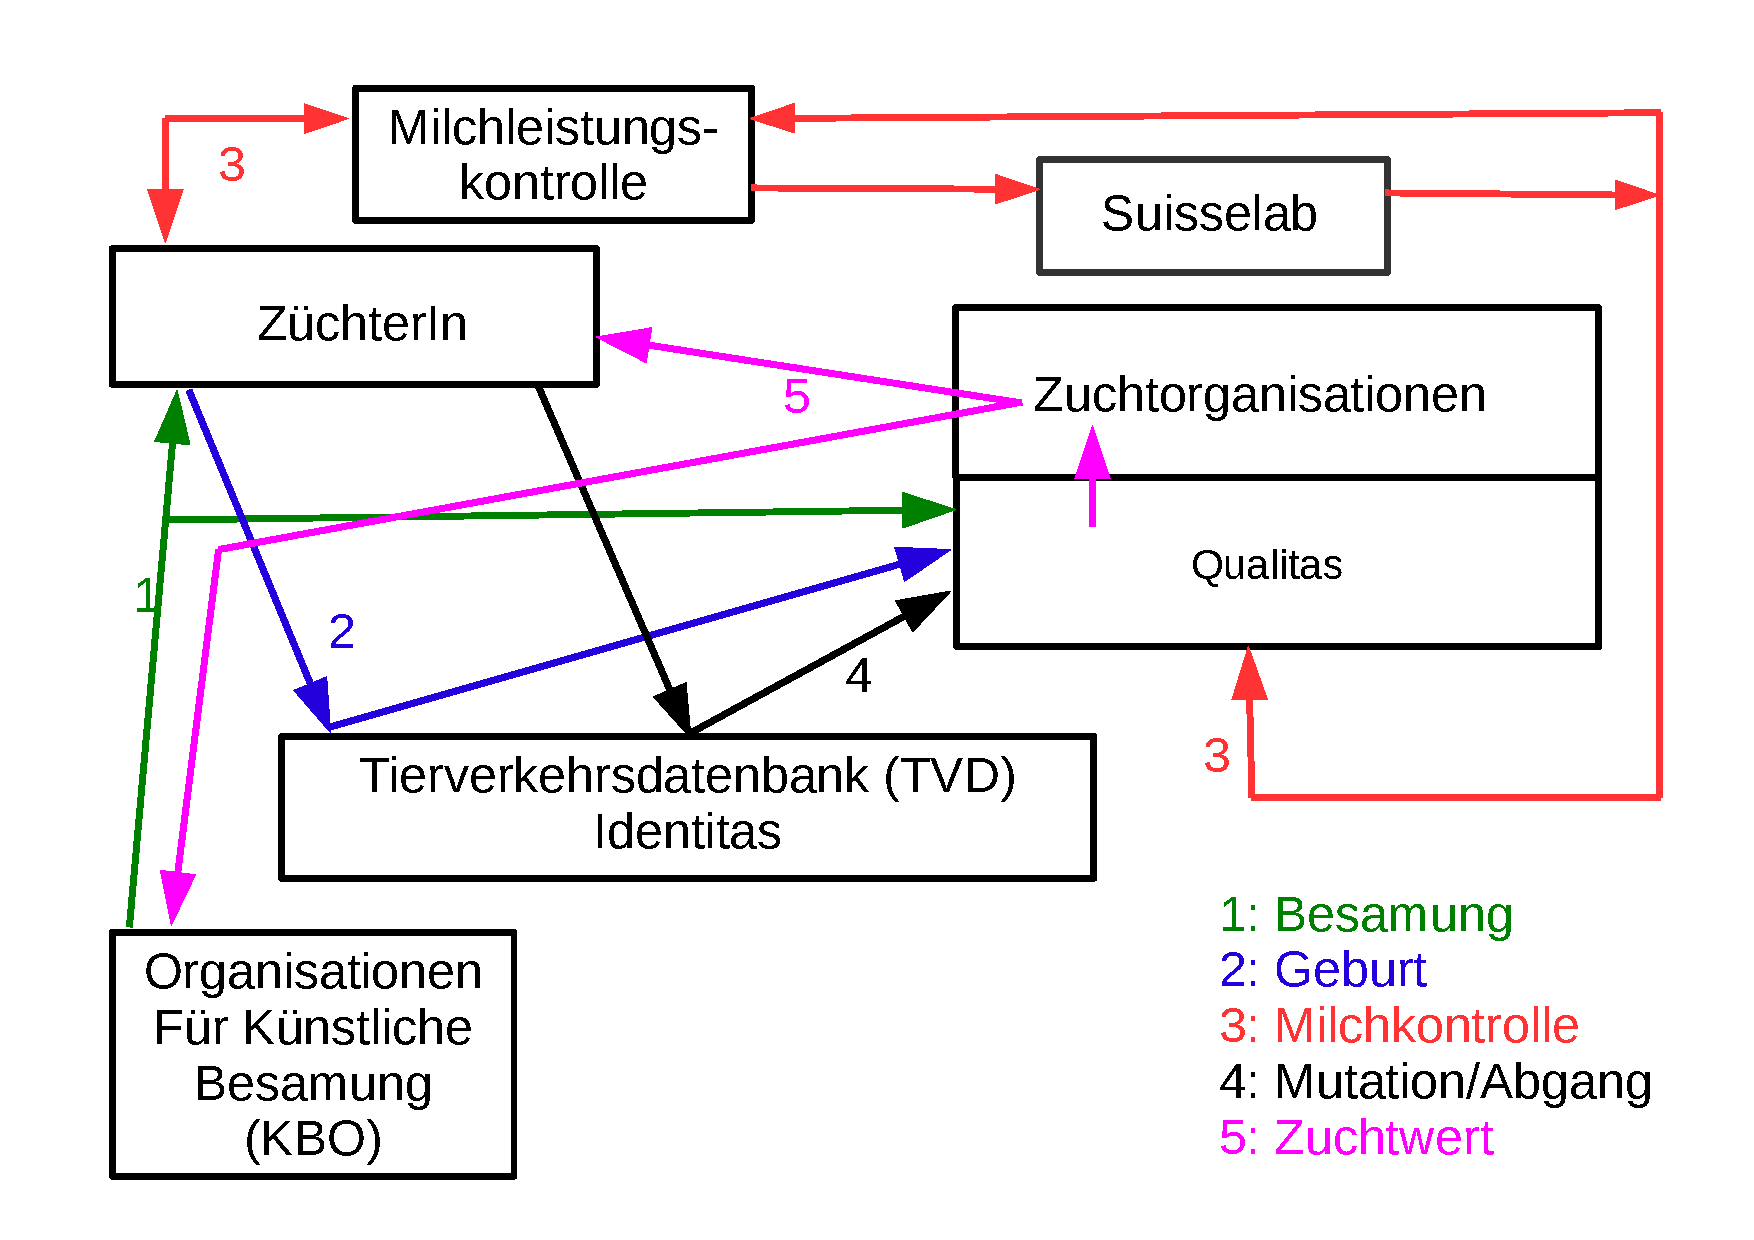
\includegraphics{ZuchtprogrammKomplett} \end{center}

\subsection{Paradigmenwechsel}\label{paradigmenwechsel}

Die Publikation \citep{MHG2001} gilt als Grundstein für eine neue Ära in
der praktischen Zuchtarbeit. Die Autoren haben gezeigt, wie genomische
Information, welche in genügender Dichte vorliegen muss, zur Schätzung
von Zuchtwerten verwendet werden kann. Sie konnten auch statistische
Methoden zeigen, mit welchen die Parameter in verwendeten Modell
geschätzt werden können. Wir werden zu einem späteren Zeitpunkt noch
genauer auf den Inhalt des Papers von \citep{MHG2001} zurückkommen.

\subsection{Vor der genomischen
Selektion}\label{vor-der-genomischen-selektion}

Von Anfangs der 1980-er Jahre wurden die statistischen Auswertungen in
den Zuchtprogrammen auf das BLUP-Tiermodell abgestellt. In dieser Zeit
wurden die einfachen Modelle auch durch verschiedene Erweiterungen
ausgebaut. Bei der Milchproduktion wurde von einfachen
Laktationsleistungen auf Testtagesmodelle umgestellt. Bei der Wurfgrösse
beim Schwein oder anderen diskreten Merkmalen wurden auch
\texttt{Generalized\ Linear\ Mixed\ Models} (GLMM) verwendet. Unabhängig
von den verwendeten Modellen wurden in allen Auswertungen die gleichen
Informationen berücksichtigt. - phänotypische Leistungen - Pedigree -
Varianzkomponenten aus periodischen Schätzungen

Versuchsweise wurde ab den 1990-er Jahren erste genetische Marker mit in
den Zuchtprogrammen berücksichtigt. Das Problem war dass diese wenigen
Markern sehr schnell auf einer bestimmten Variante fixiert war. Nach der
Fixierung lieferten diese Genorte keine zusätzliche Information zur
Auswahl von potentiellen Zuchttieren. Es war zu dieser Zeit nicht klar,
wie das Problem der Fixierung von einzelnen Genorten behandelt werden
soll und es gab auch keine wirklich gute Strategie für die
Berücksichtigung von genetischen Informationen in Zuchtprogrammen.

\subsection{Modellierung vor der genomischen
Selektion}\label{modellierung-vor-der-genomischen-selektion}

Vor der Einführung der genomischen Selektion war das BLUP-Tiermodell die
Methode der Wahl für die Auswertung von Leistungsdaten in der Tierzucht.
In seiner einfachsten Form sieht dieses Modell wie folgt aus.

\begin{equation}
  y = Xb + Zu + e
\end{equation}

\begin{tabular}{lll} 
wobei  &  $y$  &  Vektor mit phänotypischen Beobachtungen\\ 
       &  $b$  & Vektor mit fixen Effekten              \\ 
       &  $X$  & Inzidenzmatrix, welche fixe Effekte den Beobachtungen zuordnet\\ 
       &  $u$  & Vektor mit Zuchtwerten (zufällig) \\ 
       &  $Z$  & Inzidenzmatrix der Zuchtwerte \\ 
       &  $e$  & Vektor mit Residuen (zufällig) 
\end{tabular}

Die Co-Varianzen der zufälligen Komponenten sind definiert als:

\[Var(\mathbf{e}) = \mathbf{R} = \mathbf{I}*\sigma_e^2\]
\[Var(\mathbf{u}) = \mathbf{G} = \mathbf{A} * \sigma_g^2\]
\[Cov(\mathbf{u},\mathbf{e}^T) = Cov(\mathbf{e}, \mathbf{u}^T) = \mathbf{0}\]
\[\rightarrow Var(\mathbf{y}) = \mathbf{V} = \mathbf{ZGZ}^T + \mathbf{R}\]

\section{Genomische Selektion}\label{gensel}

Vom Standpunkt der Genetik aus basiert das BLUP-Tiermodell auf dem
sogenannten Infinitesimalmodell. In diesem Modell wird angenommen, dass
die phänotypische Ausprägung eines Merkmals durch die Summe von
unendlich vielen Genorten mit undendlich kleiner Wirkung verursacht
wird. Durch diese Annahme lässt sich dem einzelnen Tier kein fix
definierter Genotyp mehr zuordnen. Diese fehlende Zuordnung der
einzelnen Genotypen wird über die Modellierung der Zuchtwerte als
zufällige Effekte gelöst. Die zufälligen Effekte der Zuchtwerte
entsprechen dabei Realisierungen einer Zufallsvariablen mit vorgegebener
Verteilung.

In der genomischen Selektion verwenden wir das polygene Modell. Dabei
werden die phänotypischen Leistungen als Summe von bekannten Genorten
zusammengesetzt. Die konkrete Umsetzung des polygenen Modells wurde zum
ersten Mal im Paper von \citep{MHG2001} gezeigt. Diese Autoren haben
aufgrund von simulierten Daten gezeigt, dass es mit Hilfe einer sehr
dichten Markerkarte möglich ist, die phänotypischen Leistungen alleine
aufgrund der geschätzten Wirkungen an den Markergenorten zu modellieren.

Die folgende Abbildung fasst die Unterschiede zwischen dem
Infinitesimalmodell und dem polygenen Modell zusammen.

\begin{center}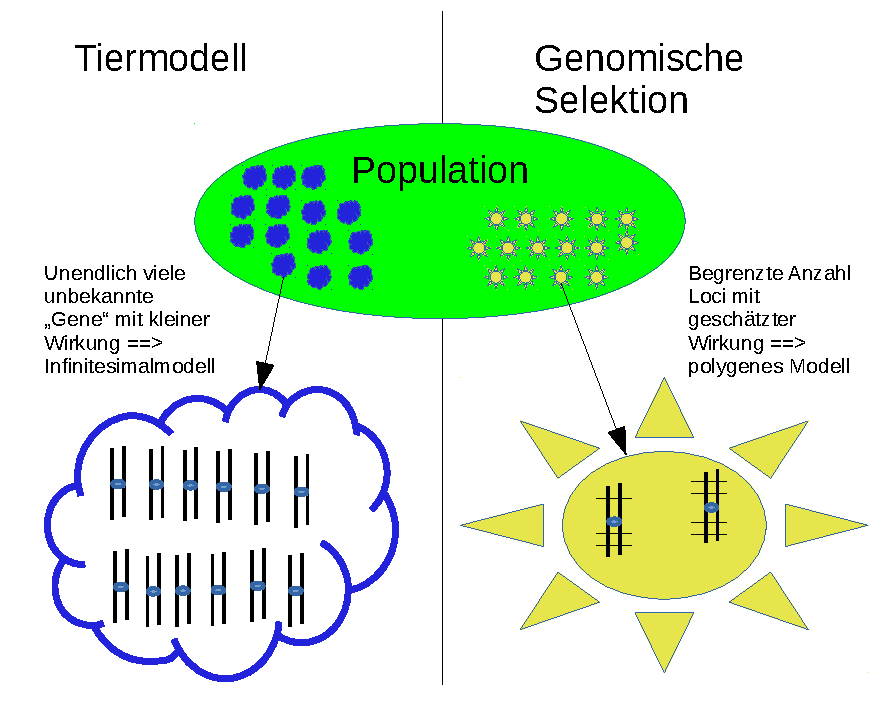
\includegraphics{AnimalModelVsGenomicSelection} \end{center}

\subsection{Modellierung}\label{modellierung}

Im Zusammenhang mit der genomischen Selektion besteht die Modellierung
der Daten aus zwei Komponenten

\begin{enumerate}
\def\labelenumi{\arabic{enumi}.}
\tightlist
\item
  Die Schätzung der Gen-Wirkungseffekte (\(a\))
\item
  Die Schätzung der genomischen Zuchtwerte
\end{enumerate}

Die Umsetzung der beiden Komponenten wird in zwei verschiedenen
Verfahren gemacht. Im Zwei-Schritt-Verfahren werden beide Komponenten
einzeln an verschiedenen Teilen der Zuchtpopulation ausgeführt. Im
Gegensatz dazu werden im Single-Step-Verfahren beide Komponenten im
gleichen Schritt realisiert.

\subsection{Zwei-Schritt-Verfahren}\label{zwei-schritt-verfahren}

Beim Zwei-Schritt-Verfahren wird die Population in ein Trainings- und
ein Testset unterteilt. Im Trainingsset werden aufgrund von
Typisierungsergebnissen und Beobachtungen die Gen-Wrkungseffekte (\(a\))
geschätzt. Sobald die Schätzwerte für die \(a\)-Effekte bekannt sind
können diese für die Schätzung der genomischen Zuchtwerte verwendet
werden.

Da aufgrund der Typisierungsergebnisse die Genotypen an den SNP-Genorten
bekannt sind, brauchen wir kein gemischtes lineares Modell mehr. Im
Gegensatz zur BLUP-Zuchtwertschätzung, ist in der genomischen Selektion
beim Zwei-Schritt-Verfahren ein einfaches lineares Modell ausreichend.
Im Idealfall, wenn die komplette Information zu allen
Gen-Wirkungseffekten (\(a\)) bekannt sind, dann setzen sich die
genotypischen Werte einfach zusammen aus den aufsummierten \(a\)-Werten.
In Matrix-Vektor-Schreibweise können wir die folgende Modellgleichung
aufstellen.

\begin{equation}
  g = 1\mu + Ma + \epsilon
\end{equation}

\begin{tabular}{lll}
wobei:  &  $g$         &  Vektor von wahren genomischen Zuchtwerten \\
        &  $\mu$       &  Achsenabschnitt \\
        &  $a$         &  Vektor mit Gensubstitutionseffekten \\
        &  $M$         &  Inzidenzmatrix als Verknüpfung zwischen $a$ und $g$ \\
        &  $\epsilon$  &  Vektor von zufälligen Residuen 
\end{tabular}

Die Matrix \(M\) ist eine Inzidenzmatrix, welche die genotypischen Werte
im Vektor \(g\) mit den Gen-Wirkungseffekten \(a\) verknüpft. Die Matrix
\(M\) hat die Dimension \(n\times p\) wobei \(n\) der Anzahl Individuen
mit einem Typisierungsergebnis entspricht und \(p\) gleich der Anzahl
SNP-Genorte ist.

In der Realität im ersten Schritt des Zwei-Schritt-Verfahrens kennen wir
aber weder die Komponenten des Vektors \(g\) noch die
Gensubstitutionseffekte \(a\). Somit müssen wir das Modell zur Schätzung
der \(a\)-Effekte modifizieren. Bei der aktuellen Modifikation ersetzen
wir den Vektor \(g\) durch die phänotypischen Beobachtung \(y\).

\begin{equation}
  y = (1\mu + Xb) + Ma + (\epsilon+ e)
\end{equation}

\begin{tabular}{lll}
wobei:  &  $y$  &  Vektor der phänotypischen Beobachtungen \\
        &  $b$  &  Vektor der fixen Umweltfaktoren \\
        &  $X$  &  Inzidenzmatrix der fixen Effekte\\
        &  $e$  &  Vektor von nicht-genetische Residuen
\end{tabular}

Das Modell mit den phänotypischen Beobachtungen erlaubt eine Schätzung
der \(a\)-Effekte. Mit diesem Ansatz gibt es aber zwei Probleme.

\begin{enumerate}
\def\labelenumi{\arabic{enumi}.}
\tightlist
\item
  \textbf{Verfügbarkeit}: wirtschaftliche Merkmale wie Milchleistung
  sind nur beim weiblichen Geschlecht beobachtbar. Somit müsste für die
  Selektion auf der männlichen Seite wieder auf Nachkommenleistungen
  zurückgegriffen werden. Dies verlängert aber das
  Generationenintervall.
\item
  \textbf{Vergleichbarkeit}: Beim Austausch von Information zwischen
  verschiedenen Ländern sind die phänotypischen Leistungen nicht
  unbedingt vergleichbar.
\end{enumerate}

Diese beiden Probleme können gelöst werden, wenn anstelle von
phänotypischen Leistungen \(y\), geschätzte Zuchtwerte \(\hat{g}\)
verwendet werden. Das entsprechende Modell sieht dann wie folgt aus.

\begin{equation}
\hat{g} = g + (\hat{g} - g) = 1\mu + Ma + (\epsilon + (\hat{g} - g) )
\end{equation}

\subsection{Eigenschaften von
BLUP-Zuchtwerten}\label{eigenschaften-von-blup-zuchtwerten}

Aufgrund der Eigenschaften von den BLUP-Zuchtwerten \(\hat{g}\) führt
die Addition der Abweichung \((\hat{g} - g)\) zu einer Reduktion der
Varianz. Die Reduktion der Varianz bedeutet, dass
\(var(\hat{g}) \le var(g)\) ist. Für BLUP-Zuchtwerte gilt, dass die
Covarianz zwischen wahrem und geschätztem Zuchtwert gleich der Varianz
der geschätzten Zuchtwerte ist. In Formeln geschrieben bedeutet dass,

\begin{equation}
  cov(\hat{g},g) = var(\hat{g})
\end{equation}

Setzen wir diese Beziehung in die Varianz der Abweichung
\((\hat{g} - g)\) ein, dann erhalten wir

\begin{equation}
  var(\hat{g} - g) = var(\hat{g}) + var(g) - 2cov(\hat{g},g) = var(g) - var(\hat{g}) \ge 0
\end{equation}

Somit gilt, dass \(var(g) \ge var(\hat{g})\) und somit ist die Reduktion
der Varianz gezeigt. Im Zusammenhang mit der Varianzreduktion steht auch
die zweite Eigenschaft von BLUP-Zuchtwerten, welche uns hier
Schwierigkeiten bereitet und zwar handelt es sich dabei um den
sogenannten Shrinkage-Effekt. Für einen geschätzten Zuchtwert eines
Tieres \(i\) bedeutet das, dass dieser zum Durchschnitt der geschätzten
Zuchtwerte der Eltern regressiert wird. Das Ausmass dieses
Regressions-Effektes hängt davon ab, aufgrund welcher Informationen der
Zuchtwert von Tier \(i\) geschätzt wurde. Diese Abhängigkeit wird in der
Zerlegung des geschätzten BLUP-Zuchtwertes des Tieres \(i\) in seine
Komponenten sichtbar. Diese Zerlegung ist in \citep{Hofer1990} und in
\citep{vonRohr2016} erklärt. Das Resultat der Zerlegung ist in der
nachfolgenden Formel zusammengefasst.

\begin{eqnarray}
\hat{g}_i &=& \frac{1}{1 + \alpha \delta^{(i)} + {\alpha\over 4} \sum_{j=1}^n \delta^{(k_j)}}
              \left[y_i - \hat{\mu} + {\alpha\over 2}\left\{\delta^{(i)}(\hat{g}_s + \hat{g}_d) 
              + \sum_{j=1}^n \delta^{(k_j)} (\hat{g}_{k_j} - {1\over 2}\hat{g}_{l_j}) \right\} \right]
\label{eq:AhatDecompEq}
\end{eqnarray}

Die Zerlegung des geschätzen Zuchtwertes \(\hat{g}_i\) für Tier \(i\)
zeigt die Abhängigkeit des Ausmasses der Regression von \(\hat{g}_i\)
auf den Durchschnitt der geschätzten Elternzuchtwerte \(\hat{g}_s\) und
\(\hat{g}_d\). Hat das Tier \(i\) keine Eigenleistung \(y_i\), keine
Nachkommen und keine Paarungspartner, so ist \(\hat{g}_i\) vollständig
durch \(\hat{g}_s\) und \(\hat{g}_d\) bestimmt. Sobald aber Tier \(i\)
eine Eigenleistung hat und später dann noch Nachkommenleistungen
dazukommen, nimmt der Einfluss von \(\hat{g}_s\) und \(\hat{g}_d\) auf
\(\hat{g}_i\) ab. Damit verringert sich auch das Ausmass des
Regressions-Effektes von \(\hat{g}_i\) auf den Durchschnitt der
geschätzten Elternzuchtwerte.

Durch die Berücksichtigung zusätzlicher Informationen, wie Eigenleistung
und Leistungen von Nachkommen und Paarungsparter, bei der Schätzung des
Zuchtwertes für Tier \(i\) steigt auch die Genauigkeit oder das
Bestimmtheitsmass (\(B\)) des geschätzten Zuchtwertes. Wir können
aufgrund der Eigenschaften von BLUP-Zuchtwerten können wir folgende
Zusammenhänge aufstellen. Je grösser die verfügbare Information für die
Schätzung eines Zuchtwertes für Tier \(i\), desto grösser ist das
Bestimmtheitsmass des geschätzten Zuchtwertes und je tiefer ist der
Regressions-Effekt des geschätzten Zuchtwertes auf den Durchschnitt der
geschätzten Zuchtwerte der Eltern und je geringer ist auch die
Varianzreduktion.

\subsection{Einsatz von BLUP-Zuchtwerten in der genomischen
Selektion}\label{einsatz-von-blup-zuchtwerten-in-der-genomischen-selektion}

Eigenschaften von BLUP-Zuchtwerten führen zu Varianzreduktion und dazu
dass geschätzte Zuchtwerte zum Durchschnitt der geschätzten Zuchtwerte
der Eltern regressiert werden. Diese beiden Effekte sind problematisch
bei der Verwendung von BLUP-Zuchtwerten für die Schätzung der
\(a\)-Effekte in der genomischen Selektion. Ein bestimmtes Tier \(i\)
hat immer die gleichen SNP-Genotypen und wir gehen davon aus, dass diese
auch immer die gleiche Wirkung auf die Ausprägung eines Phänotyps haben.
Der mit BLUP geschätzte Zuchtwert eines Tieres ändert sich aber während
seines Lebens. In der Zeitperiode der Geburt bis zur Beobachtung einer
Eigenleistung ist der geschätzte Zuchtwert durch die geschätzten
Zuchtwerte der Eltern bestimmt. Mit zunehmendem Alter werden für Tier
\(i\) mehr Informationen in der Zuchtwertschätzung berücksichtigt. Somit
ändert sich der geschätzte Zuchtwert und damit würde sich auch die
aufgrund der BLUP-Zuchtwerte geschätzten \(a\)-Effekte ändern. Das ist
aufgrund von unserer Annahme der konstanten Wirkung der \(a\)-Effekte
ein unerwünschtes Verhalten.

Die unerwünschten Veränderungen der geschätzten BLUP-Zuchtwerte werden
durch eine Prozedur namens \textbf{Deregression} korrigiert. Da sich die
Veränderungen der Zuchtwerte im wesentlichen durch eine Funktion der
Änderungen im Bestimmtheitsmass beschrieben werden kann, ist die
Deregression als Korrektur von geschätzten Zuchtwerten aufgrund deren
Bestimmtheitsmass definiert. Einzelheiten zur Deregression können dem
Paper \citep{GTF2009} entnommen werden.

\section{Zusammenfassung}\label{zusammenfassung}

Die deregressierten Zuchtwerten werden als Beobachtunen für die
Schätzung der \(a\)-Effekte im ersten Schritt des
Zwei-Schritt-Verfahrens verwendet. Die geschätzen \(a\)-Werte werden
dann verwendet um im zweiten Schritt die genomischen Zuchtwerte der
restlichen Population zu berechnen.

Die im Zwei-Schritt-Verfahren verwendeten Modelle zur Schätzung der
\(a\)-Effekte sind einfache lineare Modelle. Die Anzahl der Parameter
\(p\) in diesen Modellen entspricht der Anzahl zu schätzender
\(a\)-Werte und somit der Anzahl an SNPs pro Typisierung. Diese Anzahl
ist typischerweise bei 50K kann aber auch bis 800K anwachsen. In den
meisten Fällen ist \(p >> n\), wenn \(n\) die Anzahl typisierter Tiere
ist. Somit können wir das klassische Least Squares Verfahren für die
Schätztung der Parameter nicht verwenden.

\section{Ausblick}\label{ausblick}

Das Problem \(p >> n\) kommt heutzutage in sehr vielen Anwendungen vor.
In den nachfolgenden Kapiteln wollen wir uns ein paar Lösungsansätze
anschauen, welche uns trotz der spärlich verfügbaren Informationen in
den hoch-dimensionalen Parameterräumen, sinnvolle Schätzwerte für die
Parameter im Modell liefern kann.

\chapter{Multiple Lineare Regression}\label{linreg}

Das Material dieses Kapitels ist eine Zusammenfassung aus den
Vorlesungsunterlagen von \citep{BM2014}.

Die multiple lineare Regression ist wie folgt definiert. Jedes
Individuum \(i\) oder jedes Objekt \(i\) in einem Datensatz ist
charakterisiert durch eine \textbf{Zielgrösse} \(y_i\) und durch eine
Menge von \textbf{erklärenden Variablen}
\(\left\{x_{i,1}, x_{i,2}, \ldots, x_{i,p}\right\}\). Zusammengefasst
besteht die bekannte Information für jedes Individuum oder jedes Objekt
\(i\) aus einem Datensatz aus der folgenden Menge

\[\left\{x_{i,1}, x_{i,2}, \ldots, x_{i,p}, y_i\right\}\] Das multiple
lineare Regressionsmodell versucht die Zielgrösse bis auf einen
zufälligen Restterm \(\epsilon\) als lineare Funktion der erklärenden
Variablen auszudrücken. Unser Ziel besteht in der Schätzung der
unbekannten Parameter, welche im Regressionsmodell enthalten sind. Die
nachfolgend gezeigte Modellformel soll die Unterscheidung zwischen
erklärenden Variablen und unbekannten Parametern verdeutlichen.

\begin{equation}
y_i = \beta_i x_{i,1} + \ldots + \beta_p x_{i,p} + \epsilon_i \qquad (i = 1, \ldots, n)
\label{eq:MultLinRegForm}
\end{equation}

Fassen wir die Gleichungen über alle \((i = 1, \ldots, n)\) zusammen und
verwenden die Matrix-Vektor-Notation, so sieht das lineare Modell in
(\ref{eq:MultLinRegForm}) wie folgt aus.

\begin{equation}
y = X\beta + \epsilon
\label{eq:MultLinRegMatVec}
\end{equation}

\begin{tabular}{lll}
wobei  &              & \\
       &  $y$         &  Vektor der Länge $n$ mit allen Zielgrössen \\
       &  $\beta$     &  Vektor der Länge $p$ mit unbekannten Parametern \\
       &  $X$         &  Matrix der Dimension $n\times p$ mit erklärenden Variablen \\
       &  $\epsilon$  &  Vektor der Länge $n$ mit zufälligen Resteffekten
\end{tabular}

Die Reste \(\epsilon_i\) im Modell (\ref{eq:MultLinRegForm}) haben wir
als zufällige Effekte definiert. Somit müssen wir geeignete Annahmen zur
Dichteverteilung der \(\epsilon_i\) treffen. Meistens gehen wir davon
aus, dass die \(\epsilon_i\) unabhängig sind und der gleichen Verteilung
folgen. In der englischsprachigen Literatur wird das mit dem Begriff
\texttt{independent,\ identically\ distributed} (i.i.d.) bezeichnet. Der
Erwartungswert und die Varianz der Zufallsvariablen \(\epsilon\) sind
\(E\left[\epsilon_i \right] = 0\) und \(Var(\epsilon_i) = \sigma^2\).

\section{Beispiele für Lineare
Regressionen}\label{beispiele-fur-lineare-regressionen}

\subsection{Regression mit
Achsenabschnitt}\label{regression-mit-achsenabschnitt}

Die erste erklärende Variable wir oft als eine Konstante angenommen. Das
bedeutet, dass der erste Kolonnenvektor in der Matrix \(X\) gleich dem
Eins-Vektor ist. Die konstante erklärende Variable erlaubt es einen
sogenannten \textbf{Achsenabschnitt} anzupassen. In skalarer
Schreibweise hat das lineare Modell mit Achsenabschnitt die folgende
Form

\begin{equation}y_i = \beta_1 + \beta_2x_{i2} + \ldots + \beta_px_{ip} + \epsilon_i \qquad (i = 1,\ldots,n)\end{equation}

\subsection{Regression durch den
Ursprung}\label{regression-durch-den-ursprung}

Im Gegensatz zur Regression mit Achsenabschnitt steht die Regression
durch den Ursprung. Diese kennt keine konstante erklärende Variable. Das
Modell ohne Achsenabschnitt sieht dann wie folgt aus.

\begin{equation}y_i = \beta_1x_{i1}+ \ldots + \beta_px_{ip} + \epsilon_i \qquad (i = 1,\ldots,n)\end{equation}

\subsection{Regression mit transformierten
Variablen}\label{regression-mit-transformierten-variablen}

Regressionen können auch auf Transformationen der erklärenden Variablen
oder auf transformierte Zielgrössen angepasst werden. Als Beispiel
verwendet die sogenannte ``quadratische'' Regression die \(x_{ij}\) und
die \(x_{ij}^2\) als erklärende Variablen. Das Modell entspricht dann
einer quadratischen Funktion in den \(x_j\) ist aber immer noch eine
lineare Funktion im Bezug auf die Parameter \(\beta_j\).

\begin{equation}y_i = \beta_1 + \beta_2 x_{i2} + \beta_3 x_{i2}^2 + \epsilon_i \qquad (i = 1,\ldots,n)\end{equation}

Abgesehen von der quadratischen Regression sind auch andere Arten von
Transformationen der erklärenden Variablen denkbar. Ein Beipsiel ist in
der folgenden Gleichung gezeigt.

\begin{equation}y_i = \beta_i + \beta_2 \log(x_{i2}) + \beta_3 sin(\pi x_{i3}) + \epsilon_i \qquad (i = 1,\ldots,n)\end{equation}

Auch dieses Modell ist \emph{linear} in den Parametern \(\beta_j\) und
wird somit als lineare Regression bezeichnet.

\subsection{Anwendungen in den
Nutztierwissenschaften}\label{anwendungen-in-den-nutztierwissenschaften}

Eine Anwendung der linearen Regression in den Nutztierwissenschaften ist
die Schätzung vom Lebendgewicht von Tieren aufgrund des Brustumfangs.
Dafür werden Messbänder verwendet, welche auf der einen Seite den
Brustumfang angeben und auf der anderen Seite das geschätzte
Körpergewicht. Diese Anwendung macht eine Voraussage der Zielgrösse
\texttt{Körpergewicht} aufgrund der beobachteten erklärenden Variablen
\texttt{Brustumfang}.

Damit eine Voraussage für die Zielgrösse aufgrund der erklärenden
Variablen möglich ist, muss zuerst ein angemessener Datensatz vorliegen,
in welchem man für jedes Tier beide Informationen, also sowohl
Körpergewicht als auch Brustumfang bekannt ist. Aufgrund dieser
Informationen können dann die unbekannten Parameter geschätzt werden.
Die geschätzten Parameter werden dann für die Vorhersagen verwendet.

Bei diesem ersten Beispiel handelt es sich um eine einfache lineare
Regression. Das verwendete Regressionsmodelle hat nur eine erklärende
Variable (\texttt{Brustumfang}) und eine Zielvariable
(\texttt{Gewicht}). Das zu dieser Anwendung zugehörige Modell lautet

\begin{equation}y_{G,i} = \beta_1 + \beta_2 x_{B,i} + \epsilon_i\end{equation}

\subsection{Ziele der linearen
Regression}\label{ziele-der-linearen-regression}

\begin{itemize}
\item
  \textbf{Gute Anpassung}: das Modell soll so sein, dass die erklärenden
  Variablen möglichst präzise Voraussagen zu den Zielvariablen machen.
  Das Standardtool für die Anpassung ist die Methode der kleinsten
  Quadrate (\texttt{Least\ Squares}).
\item
  \textbf{Parameterschätzung}: die unbekannten Parameter sollen so
  geschätzt sein, dass eine Veränderung der erklärenden Variablen in
  einer entsprechenden Veränderung der Zielgrösse führt.
\item
  \textbf{Vorhersage}: noch nicht beobachtete Zielgrössen sollen als
  Funktionen von erklärenden Variablen vorhergesagt werden können
\item
  \textbf{Fehler und Signigikanz}: werden durch Vertrauensintervalle und
  statistische Tests beurteilt
\item
  \textbf{Modellentwicklung}: ist ein interaktiver Prozess, welche durch
  die oben genannten Ziele beeinflusst wird
\end{itemize}

\section{Methode der kleinsten Quadrate (Least
Squares)}\label{methode-der-kleinsten-quadrate-least-squares}

Gegeben sei das lineare Modell \(y = X\beta + \epsilon\). Wir wollen
eine, gemäss den oben formulierten Zielen, möglichst gute Schätzung für
\(\beta\) finden. Die folgende Darstellung erklärt, wie die Methode der
kleinsten Quadrate funktioniert.

\begin{center}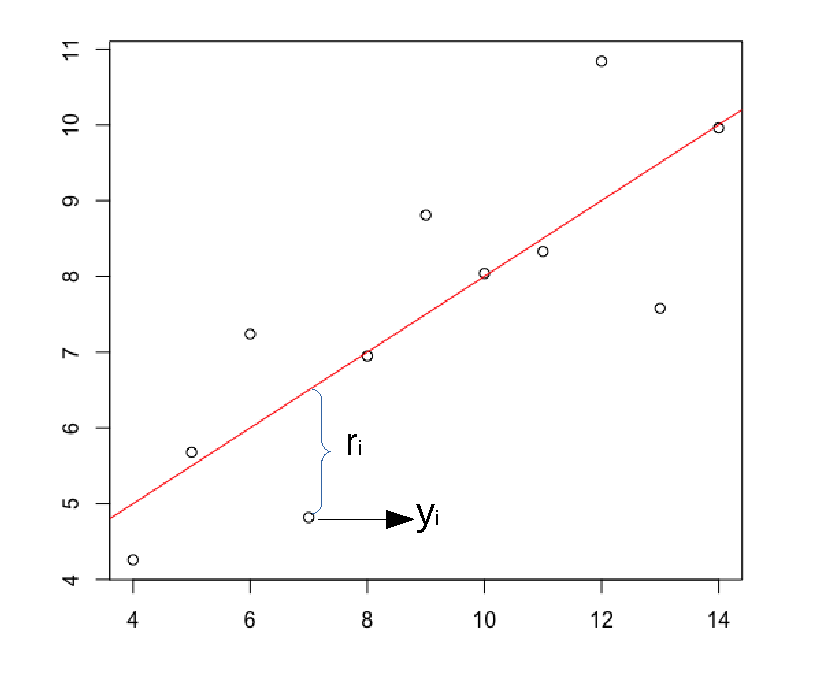
\includegraphics{LsqExplain} \end{center}

Die Punkte stehen für die Beobachtungen \(y_i\). Die rote Linie steht
für die Regressionsgerade. Die Distanz des Punktes zur Projektion in
Richtung der \(y\)-Achse auf der Regressionslinie entspricht dem
Residuum \(r_i = y_i - x_i^T \hat{\beta}\). Für eine bestimmte
Regressionsgerade (rote Linie im Diagramm) wird für jeden Punkt \(y_i\)
das entsprechende Residuum \(r_i\) berechnet. Die Residuen \(r_i\)
werden quadriert und addiert. Diese summierten Quadrate der Residuen
stellt ein Mass dar, wie gut die Regressionsgerade an die
Beobachtungspunkte \(y_i\) angepasst ist.

Position und Verlauf der Regressionsgeraden können durch die Wahl des
Vektors \(\beta\) beeinflusst werden. Gemäss der Methode der kleinsten
Quadrate soll \(\beta\) so bestimmt werden, dass die Summe der
quadrierten Residuen minimal wird. Der so bestimmte Vektor \(\beta\)
wird dann als Least-Squares-Schätzer bezeichnet. In einer Formel können
wir die Berechnung des Least-Squares-Schätzers (\(\hat{\beta}\)), wie
folgt ausdrücken.

\begin{equation}\hat{\beta} = argmin_{\beta} \| y - X\beta \| ^2\end{equation}

wobei \(\| .\|\) für die Euklidsche Norm oder die Euklidsche Distanz
steht. In einem ersten Schritt geht es darum das Minimum für den
Ausdruck \(\| y - X\beta \| ^2\) zu finden. Dabei ist es einfacher, wenn
wir folgende Umformung verwenden.

\begin{equation}\| y - X\beta \| ^2 = (y - X\beta)^T(y - X\beta) = y^Ty - y^TX\beta - \beta^TX^Ty + \beta^TX^TX\beta\end{equation}

Leiten wir diesen Ausdruck nach \(\beta\) ab und setzen die erste
Ableitung gleich \(0\), dann erhalten wir eine Gleichung für den
Least-Squares-Schätzer \(\hat{\beta}\).

\begin{equation}-y^TX - y^TX + 2\hat{\beta}^TX^TX = 0\end{equation}

Aus der obigen Formel können wir die sogenannte \textbf{Normalgleichung}
herleiten. Diese lautet

\begin{equation}X^TX\hat{\beta} = X^Ty\end{equation}

Unter der Annahme, dass die Matrix \(X\) vollen Kolonnenrang \(p\) hat,
können wir explizit nach \(\hat{\beta}\) auflösen.

\begin{equation}\hat{\beta} = (X^TX)^{-1}X^Ty\end{equation}

Die Residuen \(r_i = y_i - x_i^T\hat{\beta}\) sind Schätzungen für die
Resteffekte \(\epsilon_i\) und können somit für die Schätzung von
\(\sigma^2\) verwendet werden.

\begin{equation}\hat{\sigma}^2 = \frac{1}{n-p}\sum_{i=1}^{n} r_i^2\end{equation}

Der Faktor \(1/(n-p)\) scheint ungewöhnlich, aber es kann gezeigt
werden, dass die Wahl dieses Faktors zur Erwartungstreue von
\(\hat{\sigma}^2\) führt. Das heisst, es gilt
\(E\left[ \hat{\sigma}^2 \right] = \sigma^2\).

\subsection{Annahmen hinter dem linearen
Modell}\label{annahmen-hinter-dem-linearen-modell}

Abgesehen davon, dass die Matrix \(X\) vollen Kolonnenrang \(p<n\) haben
muss, wurden für die erklärenden Variablen keine Annahmen getroffen.
Insbesondere können die erklärenden Variablen kontinuierlich oder
diskret sein. Kontinuierliche Variablen sind typischerweise Messgrössen,
welche als reelle Zahlen (Gleitkommazahlen) erhoben werden. Diskrete
Grössen können nur bestimmte Werte, wie zum Beispiel \(0\) oder \(1\)
annehmen.

Damit die Anpassung eines linearen Modells mit der Methode der kleinsten
Quadrate Sinn macht und die Tests und Vertrauensintervalle gültig sind,
müssen wir gewisse Annahmen treffen.

\begin{enumerate}
\def\labelenumi{\arabic{enumi}.}
\tightlist
\item
  \textbf{Korrektheit des linearen Modells}: Das heisst
  \(E\left[\epsilon_i \right] = 0\) für alle \(i\). Das heisst aber
  auch, dass die Zielgrössen und die erklärenden Variablen nicht
  gemischt werden dürfen.
\item
  \textbf{Alle \(x_i\) sind exakt}: Es wird angenommen, dass die Werte
  für \(x_i\) ohne Fehler beobachtet werden können.
\item
  \textbf{Konstante Varianz der Resteffekte}:
  \(Var(\epsilon_i) = \sigma^2\) für alle \(i\)
\item
  \textbf{Resteffekte sind unkorreliert}:
  \(Cov(\epsilon_i, \epsilon_j) = 0\) für alle \(i\ne j\)
\item
  \textbf{Resteffekte folgen Normalverteilung}: Der Vektor \(\epsilon\)
  der Resteffekte folgt einer multivariaten Normalverteilung.
\end{enumerate}

Falls diese Annahmen verletzt sind, gibt es eine Reihe von Massnahmen,
welche getroffen werden können. Bei Verletzung der Annahme 3, können
``weighted least squares'' Methoden verwendet werden. Ähnlich bei
Verletzung der Annahme 4, können wir ``generalized least squares''
verwenden. Ist die Annahme 5 der Normalverteilung nicht erfüllt, können
wir auf sogenannte ``robuste Methoden'' ausweichen. Falls Annahme 2
nicht zutrifft, braucht es Korrekturen, welche als ``errors in
variables'' bezeichnet wird. Falls die Annahme 1 nicht stimmt, braucht
es nicht-lineare Modelle.

Die folgende Grafik zeigt das Beispiel des sogenannten
``Pillen-Knicks''. Dabei werden die Anzahl Geburten seit 1930 in der
Schweiz gezeigt. Hier sind die Annahmen 1 und 4 verletzt. Dieses
Beispiel zeigt auch die Gefahr bei Vorhersagen in Bereiche, wo keine
erklärende Variablen vorliegen.

\begin{center}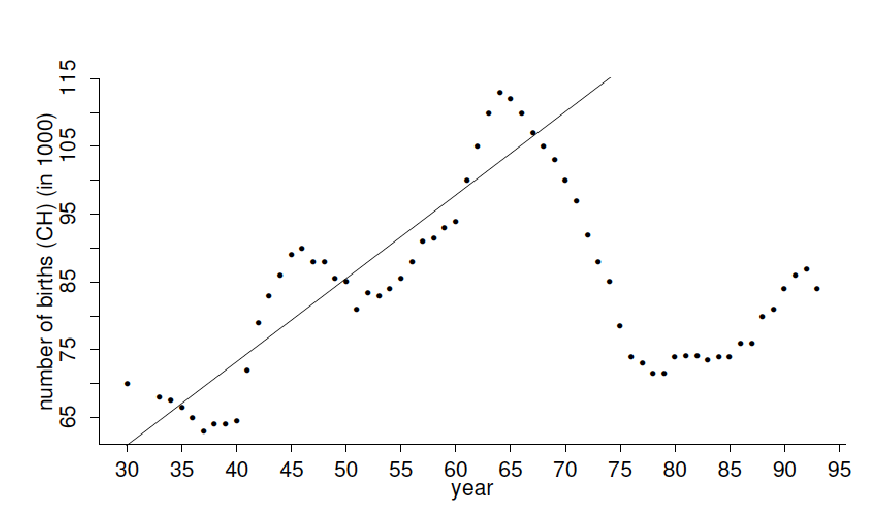
\includegraphics{PillKink} \end{center}

\subsection{Kein Ersatz der multiplen Regression durch mehrere einfache
Regressionen}\label{kein-ersatz-der-multiplen-regression-durch-mehrere-einfache-regressionen}

Eine multiple Regression (mit mehreren erklärenden Variablen) soll nicht
durch mehrere einfache Regressionen (mit nur einer erklärenden
Variablen) ersetzt werden. Das folgende simulierte Beispiel zeigt
weshalb.

Wir betrachten die folgenden erklärenden Variablen \(x^{(1)}\) und
\(x^{(2)}\) und die Zielgrösse \(y\) mit folgenden Werten

\begin{center}


\begin{tabular}{r|r|r}
\hline
x1 & x2 & y\\
\hline
0 & -1 & 1\\
\hline
1 & 0 & 2\\
\hline
2 & 1 & 3\\
\hline
3 & 2 & 4\\
\hline
0 & 1 & -1\\
\hline
1 & 2 & 0\\
\hline
2 & 3 & 1\\
\hline
3 & 4 & 2\\
\hline
\end{tabular}
\end{center}

Die multiple Regression führt zur Lösung der kleinsten Quadrate, welche
die Daten exakt beschreibt, so wie diese erzeugt wurden.

\begin{equation}y_i = \hat{y_i} = 2x_{i1} - x_{i2} \qquad \text{für alle } i \text{ mit } \hat{\sigma}^2 = 0\end{equation}

Wird an die Daten nur eine einfache Regression mit der erklärenden
Variablen \(x^{(2)}\) und ignoriert \(x^{(1)}\), so erhalten wir das
folgende Resultat

\begin{equation}\hat{y_i} = {1\over 9}x_{i2} + {4\over 3} \qquad \text{für alle } i \text{ mit } \hat{\sigma}^2 = 1.72\end{equation}

Der Grund dafür ist, dass die erklärenden Variablen \(x^{(1)}\) und
\(x^{(2)}\) korreliert sind. Falls \(x^{(1)}\) steigt, dann steigt auch
\(x^{(2)}\). Da aber in der multiplen Regression \(x^{(1)}\) einen
grösseren Koeffizienten hat als \(x^{(2)}\), muss dieser Effekt in der
einfachen Regression durch \(x^{(2)}\) kompensiert werden. Dies führt
zur Abweichung zwischen den Resultaten der beiden Analysen.

\section{Eigenschaften der
Schätzungen}\label{eigenschaften-der-schatzungen}

Die Least-Squares-Schätzer sind Zufallsvariablen, da für jeden Datensatz
den wir vom gleichen unterliegenden Prozess beobachten, andere Werte
resultieren. Damit ändern sich auch die Least-Squares-Schätzer. Da die
Schätzer Funktionen der beobachteten Daten sind, haben die Schätzer auch
einen zufälligen Charakter. Somit können wir Eigenschaften betreffend
den Verteilungen und den Momenten für die Least-Squares-Schätzer
herleiten. Die Ergebnisse sind hier nur kurz zusammengefasst.

\subsection{Momente der Least-Squares
Schätzungen}\label{momente-der-least-squares-schatzungen}

Wir nehmen das folgende lineare Modell an

\begin{equation}y = X\beta + \epsilon \text{, } E\left[\epsilon \right] = 0 \text{, } Cov(\epsilon) = E\left[\epsilon\epsilon^T \right] = \sigma^2I_{n\times n}\end{equation}

Zusammen mit den oben getroffenen Annahmen können wir folgende Aussagen
machen

\begin{enumerate}
\def\labelenumi{\arabic{enumi}.}
\tightlist
\item
  \(E\left[\hat{\beta}\right] = \beta\), das heisst, \(\hat{\beta}\) ist
  unverzerrt
\item
  \(E\left[\hat{y}\right] = E\left[y\right] = X\beta\), was aus 1.
  folgt. Zudem ist, \(E\left[r\right] = 0\)
\item
  \(Cov(\hat{\beta}) = \sigma^2(X^TX)^{-1}\)
\item
  \(Cov(\hat{y}) = \sigma^2P\), \(Cov(r) = \sigma^2(I-P)\)
\end{enumerate}

Die Matrix \(P\) ist definiert als Projektionsmatrix aus
\(\hat{y} = Py\). Setzen wir die Least-Squares-Schätzer ein, dann folgt

\begin{equation}\hat{y} = X\hat{\beta} = X(X^TX)^{-1}X^Ty = Py\end{equation}

Somit ist die Matrix \(P\) definiert als \(P=X(X^TX)^{-1}X^T\).

\subsection{Verteilung der Least-Squares-Schätzer unter normalverteilten
Fehlern}\label{verteilung-der-least-squares-schatzer-unter-normalverteilten-fehlern}

Zusätzlich zum linearen Modell nehmen wir an, dass
\(\epsilon_i, \ldots, \epsilon_n \text{ i.i.d. } \mathcal{N}(0,\sigma^2)\),
dann können wir zeigen, dass

\begin{enumerate}
\def\labelenumi{\arabic{enumi}.}
\tightlist
\item
  \(\hat{\beta} \sim \mathcal{N}_p\left(\beta, \sigma^2(X^TX)^{-1}\right)\)
\item
  \(\hat{y} \sim \mathcal{N}_n\left(X\beta,\sigma^2P \right)\),
  \(r \sim \mathcal{N}_n\left(0,\sigma^2(I-P) \right)\)
\item
  \(\hat{\sigma}^2 \sim \frac{n}{n-p}\chi_{n-p}^2\)
\end{enumerate}

Die Annahme der Normalverteilung ist oft (annähernd) erfüllt und kann
durch den zentralen Grenzwertsatz bei grösseren Datensätzen begründet
werden. Diese Eigenschaften im Bezug auf die Verteilung der Schätzer
führt zur Herleitung von Vertrauensintervallen und statistischen Tests
für die geschätzten Parameter. Sind die Annahmen der Normalverteilung
nicht erfüllt, müssen wir auf sogenannte robuste Methoden ausweichen.
Diese werden hier nicht behandelt.

\section{Tests und
Vertrauensintervalle}\label{tests-und-vertrauensintervalle}

\subsection{Einzeltests}\label{einzeltests}

Wir nehmen an, dass das lineare Modell korrekt ist und dass die
Resteffekte
\(\epsilon_1, \ldots, \epsilon_n \text{ i.i.d. } \sim \mathcal{N}\left(0, \sigma^2 \right)\).
Dann haben wir gesehen gemäss den Eigenschaften aus dem vorherigen
Abschnitt ist dann \(\hat{\beta}\) normalverteilt.

Im Allgemeinen sind wir daran interessiert, ob ein bestimmter Parameter
\(\beta_j\) einen Einfluss hat. Dies lässt sich mit der Nullhypothese
\(H_{0,j}: \beta_j = 0\) gegenüber der Alternativen
\(H_{A,j}: \beta_j \ne 0\) überprüfen. Da \(\hat{\beta}\) einer
Normalverteilung folgt, können wir herleiten, dass unter der
Nullhypothese \(H_{0,j}\) gilt

\begin{equation}\frac{\hat{\beta_j}}{\sqrt{\sigma^2(X^TX)_{jj}^{-1}}} \sim \mathcal{N}(0,1)\end{equation}

Da \(\sigma^2\) unbekannt ist, ist die obige Teststatistk in der Praxis
nicht brauchbar. Ersetzen wir \(\sigma^2\) durch den Schätzwert
\(\hat{\sigma}^2\) so erhalten wir die sogenannte t-Teststatistik.

\begin{equation}T_j = \frac{\hat{\beta_j}}{\sqrt{\hat{\sigma}^2(X^TX)_{jj}^{-1}}} \sim t_{n-p}\end{equation}

Anhand dieses Tests können wir die Relevanz der erklärenden Variablen
quantifizieren, indem wir die Teststatistiken \(T_j\) für
\(j=1,\ldots,p\) analysieren. Die Beurteilung der Relevanz der
erklärenden Variablen aufgrund dieser einzelnen t-Tests birgt zwei
Probleme.

\begin{enumerate}
\def\labelenumi{\arabic{enumi}.}
\tightlist
\item
  \textbf{Multiples Testen}: Werden sehr viele Tests durchgeführt, dann
  sind bei einem angenommenen Signifikanz-Niveau von \(\alpha\)
  automatisch ein Anteil \(\alpha\) aller Tests signifikant. Werden
  beispielsweise \(100\) Tests auf dem Niveau \(\alpha = 0.05\)
  durchgeführt, dann sind automatisch \(5\) Tests signifikant.
\item
  \textbf{Korrelation der erklärenden Variablen}: Falls die erklärenden
  Variablen untereinander korreliert sind, dann beeinflusst dies auch
  die Testergebnisse und kann diese verzerren.
\end{enumerate}

\subsection{Globaler Test}\label{globaler-test}

Wenn wir testen wollen, ob (abgesehen vom Achsenabschnitt) überhaupt
eine erklärende Variable einen Einfluss auf die Zielgrösse hat, dann
können wir diese mit folgender Nullhypothese
\(H_0: \beta_2 = \ldots = \beta_p = 0\) versus die Alternative
\(H_A: \beta_j \ne 0\) für \(j=2,\ldots, p\) tun. Solch ein Test kann
mit der Zerlegung der Varianz der Beobachtungen \(y_i\) um das globale
Mittel \(\bar{y} = n^{-1}\sum_{i=1}^ny_i\) konstruiert werden. In
Vektor-Schreibweise sieht diese Zerlegung wie folgt aus

\begin{equation}\|y - \bar{y}\|^2 = \|\hat{y} - \bar{y}\|^2 + \|y - \hat{y}\|^2\end{equation}

Diese Zerlegung teilt die quadrierten Abweichungen der Beobachtungen
\(y\) vom allgemeinen Mittel \(\bar{y}\) in die quadrierten Abweichungen
der gefitteten Werte \(\hat{y}\) vom allgemeinen Mittel plus die
quadrierten Residuen \(y-\hat{y}\) auf. Eine solche Zerlegung lässt sich
am einfachsten in einer Varianzanalysetabelle zusammenfassen.

\begin{center}

\begin{tabular}{llll}
\hline
            &   Summenquadrate             &  Freiheitsgrade &  mittlere Summenquadrate          \\
\hline
Regression  &   $\|\hat{y} - \bar{y}\|^2$  &  $p-1$          &  $\|\hat{y} - \bar{y}\|^2/(p-1)$  \\
Rest        &   $\|y - \hat{y}\|^2$        &  $n-p$          &  $\|y - \hat{y}\|^2/(n-p)$        \\
\hline
Total       &   $\|y - \bar{y}\|^2$        &  $n-1$          &
\end{tabular}
\end{center}

Im Falle der globalen Nullhypothese haben die erklärenden Variablen
keinen Einfluss auf die Zielgrösse. Somit ist
\(E\left[y \right] = const. = E\left[\bar{y}\right]\). Daraus folgt,
dass der Erwartungswert der mittleren Summenquadrate der Regression
gleich \(\sigma^2\) ist. Teilen wir die mittleren Summenquadrate der
Regression durch die mittleren Summenquadrate des Rests (Schätzung von
\(\sigma^2\)) erhalten wir eine dimensionslose Grösse, welcher einer
\(F\)-Statistik entspricht. Unter der Nullhypothese gilt, dass

\begin{equation}F = \frac{\|\hat{y} - \bar{y}\|^2/(p-1)}{\|y - \hat{y}\|^2/(n-p)} = F_{p-1,n-p}\end{equation}

Dies wird als globaler \(F\)-Test der Regression bezeichnet.

Abgesehen von der Bewertung der statistischen Signifikanz mit dem
globalen \(F\)-Test, sind wir auch daran interessiert, wie gut die
Anpassung des Modells an die Daten ist. Eine mögliche Grösse für die
Qualität der Anpassung ist das sogenannten \(R^2\). Dies ist definiert
als das folgende Verhältnis.

\begin{equation}R^2 = \frac{\|\hat{y} - \bar{y}\|^2}{\|y - \bar{y}\|^2}\end{equation}

Das \(R^2\) entspricht dem Verhältnis der Variation der Beobachtungen um
das globale Mittel, welcher durch die Regression erklärt werden kann.
Aus dieser Definition ist klar, dass wir nach Modellen suchen mit einem
möglichst grossen \(R^2\).

\subsection{Vertrauensintervalle}\label{vertrauensintervalle}

In Anlehnung an den \(t\)-Test der einzelnen Parameter \(\beta_j\)
können wir Vertrauensintervalle ableiten. Das zwei-seitige
Vertraunensintervall auf dem Niveau \(1-\alpha\) für \(\beta_j\) ist
definiert als

\begin{equation}\hat{\beta}_j \pm \sqrt{\hat{\sigma}^2(X^TX)_{jj}^{-1}} \ \cdot t_{n-p;1-\alpha/2}\end{equation}

Hier \(t_{n-p;1-\alpha/2}\) ist das \(1-\alpha/2\)-Quantil der
\(t_{n-p}\)-Verteilung.

\section{Output von R}\label{output-von-r}

In R wird eine lineare Regression mit der Funktion \texttt{lm()}
angepasst. Die Zusammenfassung der Resultate von \texttt{lm()} ist in
der nachfolgenden Diagramm gezeigt.

\begin{center}\includegraphics{LinModResults} \end{center}

Die verschiedenen Bereiche der Resultate sind numeriert durch farbige
Rechtecke gekennzeichnet. Im ersten Bereich ist unter der Überschrift
\texttt{Call} der Funktionsaufruf nochmals aufgeführt. So ist
dokumentiert, wie die nachfolgenden Resultate zustande kamen. Der zweite
Bereich gibt einige Informationen zur empirischen Verteilung der
Residuen. Diese Kennzahlen der Residuen-Verteilung sind nützlich um
gewisse Annahmen bezüglich der Residuen im Modell grob überprüfen zu
können. Block drei enthält die Resultate der Parameterschätzungen.
Abgesehen von den Schätzwerten sind auch die Standardfehler und die
Quantile des entsprechenden t-Tests für jeden Parameter enthalten. Die
Kolonne ganz links im Block drei zeigt das Signifikanz-Niveau der
t-Tests für jeden Parameterschätzwert. Der vierte und letzte Block
enthält die Schätzung der Rest-Standardabweichung (residual standard
error) und das Testergebnis des globalen F-Tests. Zur Beurteilung der
Anpassungsqualität ist das \(R^2\) und eine korrigierte Version des
\(R^2\) aufgeführt. Die korrigierte Version des \(R^2\) berücksichtigt
die Anzahl der geschätzten Parameter und ist definiert als

\begin{equation}\bar{R}^2 = R^2 - (1-R^2)\frac{p-1}{n-p}\end{equation}

\section{Analyse der Residuen und Überprüfung der
Modellannahmen}\label{analyse-der-residuen-und-uberprufung-der-modellannahmen}

Die Residuen \(r_i = y_i - \hat{y}_i\) dienen als Annäherungen an die
unbekannten Resteffekte \(\epsilon_i\) und zur Überprüfung der
Modellannahmen.

\subsection{Tukey-Anscombe Plot}\label{tukey-anscombe-plot}

Der Tukey-Anscombe Plot ist ein graphisches Tool zur Feststellung von
Abhängigkeiten zwischen den Residuen \(r_i\) und den gefitteten Werten
\(\hat{y}_i\). Im Tukey-Anscombe Plot werden auf der x-Achse die
gefitteten Werte und auf der y-Achse die Resiuden aufgetragen.
Idealerweise sind die Resiuden zufällig verteilt und zeigen kein Muster.
In R erzeugt man den Tukey-Anscombe Plot über die Hilfsfunktionen
\texttt{fitted()} und \texttt{residuals()}. Die Ergebnisse der beiden
Funktionen werden einfach an die \texttt{plot()}-Funktion übergeben.

\begin{Shaded}
\begin{Highlighting}[]
\KeywordTok{data}\NormalTok{(}\StringTok{"anscombe"}\NormalTok{)}
\NormalTok{fit.lm.ta <-}\StringTok{ }\KeywordTok{lm}\NormalTok{(y1 ~}\StringTok{ }\NormalTok{., }\DataTypeTok{data =} \NormalTok{anscombe)}
\KeywordTok{plot}\NormalTok{(}\KeywordTok{fitted}\NormalTok{(fit.lm.ta), }\KeywordTok{residuals}\NormalTok{(fit.lm.ta))}
\end{Highlighting}
\end{Shaded}

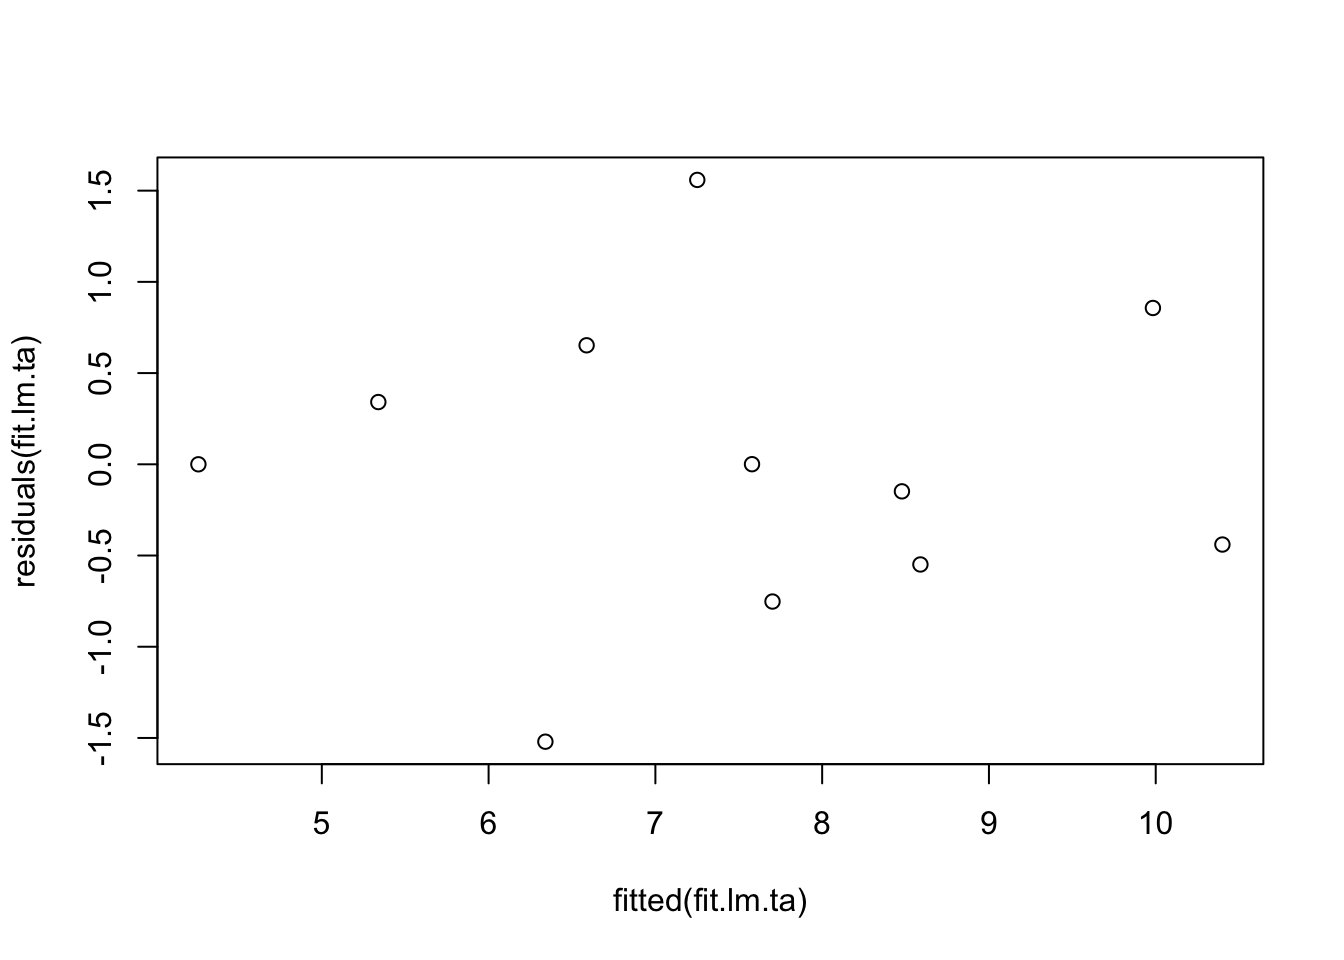
\includegraphics{bookdown-asmas_files/figure-latex/TukeyAnscombe-1.pdf}

Der obige Plot zeigt eine ideale Situation, wo keine systematischen
Muster zu erkennen sind. Die folgenden vier Plots sind \citep{BM2014}
entnommen und zeigen Probleme bei der Anpassung von linearen Modellen
auf.

\begin{center}\includegraphics{TukeyAnscombProblem} \end{center}

\subsection{Der QQ-Plot}\label{der-qq-plot}

Annahmen zur Verteilung der zufälligen Grössen im linearen Modell können
mit dem sogenannten QQ-Plot überprüft werden. Die Abkürzung ``QQ'' steht
hier für Quantil-Quantil und meint, dass wir die empirischen Quantile
den theoretischen Quantilen einer bestimmten Verteilung
gegenüberstellen. Im Fall, dass wir gegen die theoretischen Quantile
einer Normalverteilung testen, heisst der QQ-Plot auch Normal Plot.

In R können wir den QQ-Plot für die Residuen, wie folgt erzeugen.

\begin{Shaded}
\begin{Highlighting}[]
\KeywordTok{qqnorm}\NormalTok{(}\KeywordTok{residuals}\NormalTok{(fit.lm.ta))}
\KeywordTok{qqline}\NormalTok{(}\KeywordTok{residuals}\NormalTok{(fit.lm.ta))}
\end{Highlighting}
\end{Shaded}

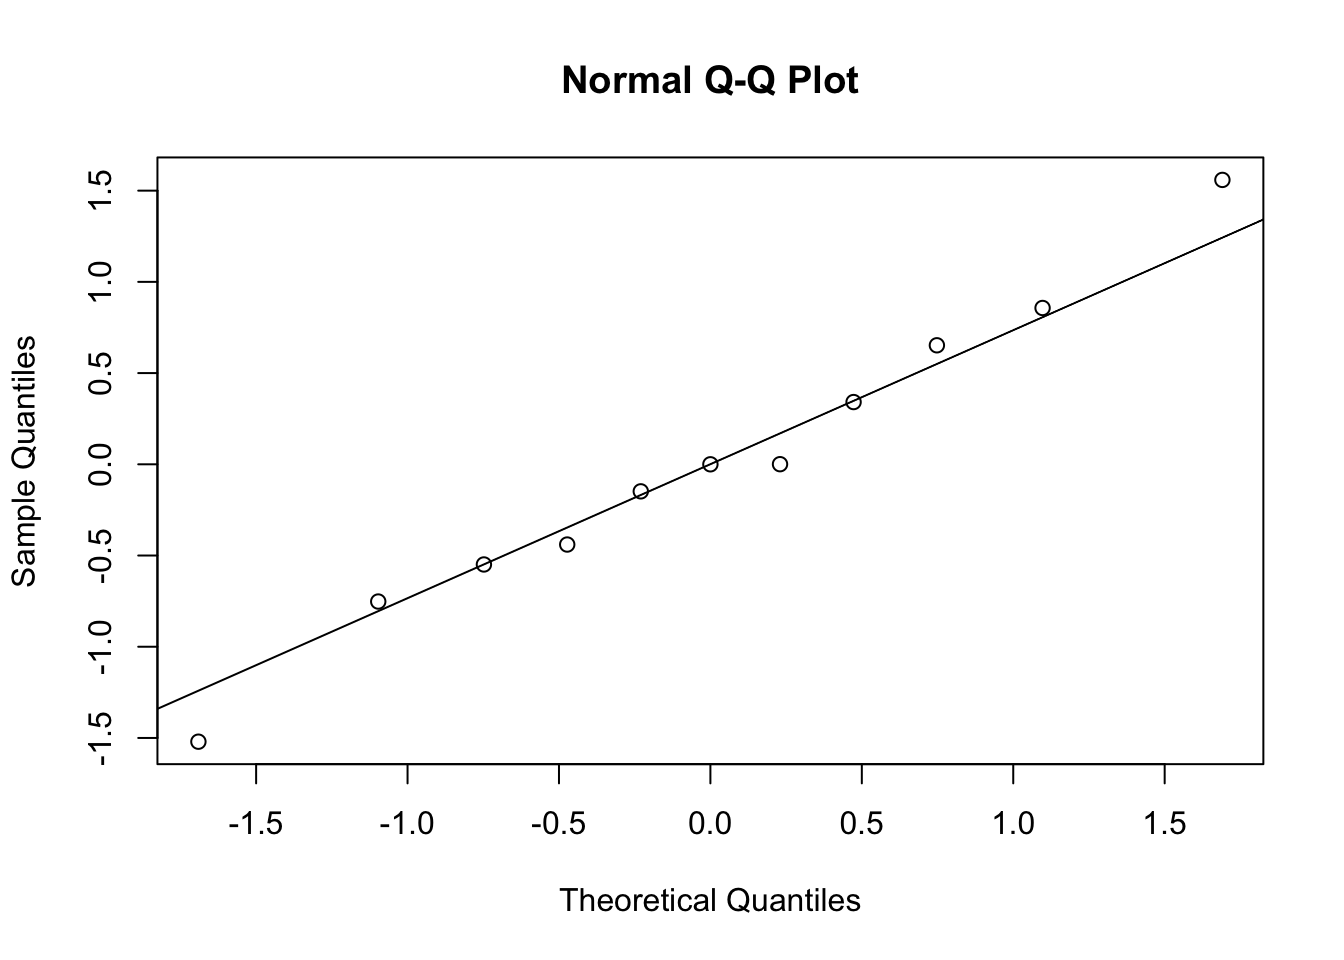
\includegraphics{bookdown-asmas_files/figure-latex/QQPlot-1.pdf}

Stimmen die Quantile der empirische Verteilung der Residuen gut mit den
theoretischen Quantilen überein, dann liegen die Punkte im QQ-Plot auf
einer Geraden. Falls die empirische Verteilung bedeutende Abweichungen
zeigt von der angenommenen Verteilung, so zeigt der Verlauf der Punkte
systematische Abweichungen, wie das in den folgenden Graphiken der Fall
ist.

\begin{center}\includegraphics{QQPlotProblems} \end{center}

\section{Selektion eines Modells}\label{selektion-eines-modells}

Gegeben sei das lineare Modell

\begin{equation}y_i = \sum_{i=1}^n \beta_j x_{ij} + \epsilon_i \quad (i = 1,\ldots,n)\end{equation}

mit \(\epsilon_1,\ldots,\epsilon_n \text{ i.i.d. }\),
\(E\left[\epsilon_i \right] = 0\) und \(Var(\epsilon_i) = \sigma^2\).

Bis anhin hatten wir immer alle erklärenden Variablen \(x_1,\ldots,x_p\)
im Modell berücksichtigt. Wir können uns aber auch fragen, ob dies Sinn
macht, wenn gewisse erklärende Variablen nicht relevant sind für die
Modellierung der Zielgrössen. Hinzu kommt noch, dass für jede erklärende
Variablen ein unbekannter Parameter \(\beta_j\) geschätzt werden muss.
Jeder geschätzte Parameter trägt zur Variabilität der gefitteten Werte
bei, ob die erklärende Variable relevant ist oder nicht. Somit wird oft
nach dem \textbf{optimalen} Modell und nicht nach dem wahren Modell
gesucht. Das optimale Modell ist definiert als das Modell mit dem
minimalen Subset an erklärenden Variablen, welche alle relevant sind für
die Modellierung der Zielgrösse.

Formell können wir das soeben Erklärte wie folgt zusammenfassen.
Angenommen, wir wollen die folgende Vorhersage, nennen wir sie
\(\mathcal{M}\), optimieren.

\begin{equation}\sum_{r=1}^q \hat{\beta}_{j_r}x_{ij_r}\end{equation}

welche die \(q\) erklärenden Variablen mit den Indices
\(j_1,\ldots,j_q \in \{1,\ldots,p\}\) enthält. Wir brauchen ein
Entscheidungskriterium um die Vorhersage \(\mathcal{M}\) mit den \(q\)
Parametern mit dem vollen Modell, welches alle erklärenden Variablen
enthält vergleichen zu können.

\subsection{\texorpdfstring{Mallows
\(C_p\)-Statistik}{Mallows C\_p-Statistik}}\label{mallows-c_p-statistik}

Die Summenquadrate der Residuen \(SSE(\mathcal{M})\) für die Vorhersage
\(\mathcal{M}\) können wir nicht als Kriterium verwenden, denn
\(SSE(\mathcal{M})\) nimmt ab mit zunehmener Anzahl \(q\) an Parametern.
Der mittlere quadrierte Fehler bei der Verwendung von \(\mathcal{M}\)
anstelle vom vollen Modell, kann als

\begin{equation}n^{-1} SSE(\mathcal{M}) - \hat{\sigma}^2 + 2\hat{\sigma}^2q/n\end{equation}

geschätzt werden, wobei \(\hat{\sigma}^2\) der geschätzte Restvarianz
aus dem vollen Modell entspricht. Da \(n\) und \(\hat{\sigma}^2\) für
alle Submodelle \(\mathcal{M}\) konstant sind, können wir als Kriterium
für den Modellvergleich die Statistik

\begin{equation}C_p(\mathcal{M}) = \frac{SSE(\mathcal{M})}{\hat{\sigma}^2} - n + 2q\end{equation}

verwenden.

\subsection{\texorpdfstring{Modellwahl mit dem
\(C_p\)-Kriterium}{Modellwahl mit dem C\_p-Kriterium}}\label{modellwahl-mit-dem-c_p-kriterium}

Für das volle Modell mit \(p\) erklärenden Variablen gibt es \(2^p-1\)
Submodelle oder Vorhersagen \(\mathcal{M}\). Somit ist ein Vergleich der
\(C_p\)-Statistik aller Submodelle nur machbar, wenn \(p\) nicht zu
gross, d.h. kleiner als \(16\) ist. Für \(p \ge 16\) werden die
folgenden zwei schrittweisen Algorithmen vorgeschlagen.

\subsubsection{\texorpdfstring{Vorwärts-Integration (``Forward
Selection) 1. Starte mit dem minimalen Modell \(\mathcal{M}_0\), welches
nur ein globales Mittel enthält 2. Wähle die erklärende Variable, welche
die Summe der quadrierten Residuen am meisten reduziert und nimm diese
ins Modell auf 3. Wiederhole Schritt 2 bis alle erklärenden Variablen im
Modell aufgenommen wurden. Das produziert eine Sequenz von Submodellen
\(\mathcal{M}_0, \mathcal{M}_1, \mathcal{M}_2, \ldots\). 4. Wähle aus
der Sequenz der Submodelle dasjenige mit dem kleinsten Wert der
\(C_p\)-Statistik}{Vorwärts-Integration (``Forward Selection) 1. Starte mit dem minimalen Modell \textbackslash{}mathcal\{M\}\_0, welches nur ein globales Mittel enthält 2. Wähle die erklärende Variable, welche die Summe der quadrierten Residuen am meisten reduziert und nimm diese ins Modell auf 3. Wiederhole Schritt 2 bis alle erklärenden Variablen im Modell aufgenommen wurden. Das produziert eine Sequenz von Submodellen \textbackslash{}mathcal\{M\}\_0, \textbackslash{}mathcal\{M\}\_1, \textbackslash{}mathcal\{M\}\_2, \textbackslash{}ldots. 4. Wähle aus der Sequenz der Submodelle dasjenige mit dem kleinsten Wert der C\_p-Statistik}}\label{vorwarts-integration-forward-selection-1.-starte-mit-dem-minimalen-modell-mathcalm_0-welches-nur-ein-globales-mittel-enthalt-2.-wahle-die-erklarende-variable-welche-die-summe-der-quadrierten-residuen-am-meisten-reduziert-und-nimm-diese-ins-modell-auf-3.-wiederhole-schritt-2-bis-alle-erklarenden-variablen-im-modell-aufgenommen-wurden.-das-produziert-eine-sequenz-von-submodellen-mathcalm_0-mathcalm_1-mathcalm_2-ldots.-4.-wahle-aus-der-sequenz-der-submodelle-dasjenige-mit-dem-kleinsten-wert-der-c_p-statistik}

\subsubsection{Rückwärts-Elimination (Backward
Selection)}\label{ruckwarts-elimination-backward-selection}

\begin{enumerate}
\def\labelenumi{\arabic{enumi}.}
\tightlist
\item
  Wir starten mit dem vollen Modell, welches alle erklärenden Variablen
  enthält
\item
  Entferne die erklärende Variable vom vollen Modell, welche die Summe
  der quadrierten Residuen am wenigsten reduziert.
\item
  Wiederhole Schritt 2 bis alle erklärenden Variablen entfernt wurden.
  Das führt zu einer Sequenz von Submodellen.
\item
  Wähle dasjenige Submodell aus der Sequenz an Submodellen mit minimaler
  \(C_p\)-Statistik
\end{enumerate}

\subsection{Bemerkungen}\label{bemerkungen}

Rückwärts-Elimination von erklärenden Variablen funktioniert im
allgemeinen besser als Vorwärts-Integration, aber ist auch teuerer im
Bezug auf Rechenleistung. In \citep{BM2014} wird die
Vorwärts-Integration für den Fall dass \(p \ge n\) als taugliche Methode
bezeichnet. Erfahrungen im Bereich der Effektschätzung in der
genomischen Selektion haben aber gezeigt, dass Vorwärts-Integration zu
keiner stabilen Prozedur für die Selektion eines guten Modells führt.

Schon die Autoren in \citep{MHG2001} haben für simulierte Daten gezeigt,
dass die Vorwärts-Integration von SNP-Effekten als erklärende Variablen
bei der Identifikation der wichtigen SNP-Effekte versagte. Offenbar gibt
es bie einer sehr grossen Anzahl von erklärenden Variablen \(p\) im
Vergleich zur Anzahl der verfügbaren Beobachtungen \(n\) das Problem,
dass im Schritt 2 der Vorwärts-Integration viele erklärende Variablen
die Summe der quadrierten Residuen um mehr oder weniger den gleich
Betrag reduzieren. Dann haben wir das Problem, dass wir eine Auswahl
zwischen fast gleichwertigen erklärenden Variablen treffen müssen. Diese
Auswahl ist offensichtlich kritisch und kann zu sehr verschiedenen
Endergebnissen in der Modellwahl führen.

\chapter{Genomic Best Linear Unbiased Prediction}\label{gblup}

\chapter{Least Absolute Shrinkage And Selection Operator
(LASSO)}\label{chpt-lasso}

Das lineare Modell

\begin{equation}
y_i = \beta_0 + \sum_{j=1}^p \beta_jx_{ij} + \epsilon_i
\label{eq:StandardLinMod}
\end{equation}

für eine Beobachtung \(i\) (\(i=1,\ldots,n\)) wird zur Modellierung von
Zusammenhängen zwischen den erklärenden Variablen
\(x_{i1},\ldots,x_{ip}\) und der Zielgrösse \(y_i\) verwendet. In einem
Regressionsmodell werden die unbekannten Parameter
\(\beta_j \ (j=0,\ldots,p)\) mit Least Squares geschätzt.

Die \((p+1)\) Werte \(\beta_0, ..., \beta_p\) und die Resteffekte
\(\epsilon_i\) sind unbekannt. Es wird angenommen, dass die Werte der
erklärenden Variablen (\(x_{i1}, x_{i2}, ..., x_{ip}\)) exakt, d.h. ohne
Messfehler oder andere Ungenauigkeiten, bekannt sind. Für einen
Datensatz mit \(n\) Beobachtungen werden die resultierenden \(n\)
Gleichungen vorzugsweise in Matrix-Vektor-Schreibweise notiert.

\begin{equation}
y = X\beta + \epsilon
\label{eq:StandardLinearModelMatrixVektor}
\end{equation}

\section{Stochastische
Restkomponente}\label{stochastische-restkomponente}

Die \(n\) unbekannten Resteffekte im Vektor \(\epsilon\) werden als
zufällige Effekte modelliert, wobei angenommen wird, dass sich diese
Resteffekte im Mittel aufheben, d.h., dass deren Erwartungswert
\(E(\epsilon) = 0\) ist. Die Streuung der Resteffekte wird im
Standardmodell als konstant angenommen. Für die Covarianz des Vektors
der Resteffekte bedeutet das, dass \(var(\epsilon) = I*\sigma^2\) ist.
Die Varianzkomponente \(\sigma^2\) ist neben den Koeffizienten im Vektor
\(\beta\) ein weiterer unbekannter Parameter, welcher von den Daten
geschätzt werden muss.

\section{Parameterschätzung}\label{parameterschatzung}

Unter der Annahme, dass die Matrix \(X\) vollen Kolonnenrang hat, d.h.
die Anzahl Beobachtungen \(n\) grösser ist als die Anzahl Parameter
(hier \(p+1\)) lassen sich die unbekannten Parameter \(\beta\) mit
\textbf{Least Squares} schätzen. Der Least Squares Schätzer
\(\hat{\beta}\) für \(\beta\) wird berechnet aus

\begin{equation}
\hat{\beta} = argmin_{\beta}||y - X\beta||^2
\label{eq:LsEstimateBeta}
\end{equation}

wobei \(||.||\) für die Euklidsche Norm (Länge) im \(n\)-dimensionalen
Raum steht. Wird das Minimierungsproblem in Gleichung
(\ref{eq:LsEstimateBeta}) aufgelöst, dann resultiert der folgende
Ausdruck für \(\hat{\beta}\)

\begin{equation}
\hat{\beta} = (X^TX)^{-1}X^Ty
\label{eq:LsEstimateBetaSol}
\end{equation}

Betrachten wir den Ausdruck in Gleichung (\ref{eq:LsEstimateBetaSol})
wird klar, weshalb die Matrix \(X\) vollen Kolonnenrang haben muss, da
nur so die Inverse \((X^TX)^{-1}\) berechnet werden kann.

\section{Alternativen zu Least
Squares}\label{alternativen-zu-least-squares}

Das lineare Modell (\ref{eq:StandardLinMod}) erweist sich in der Praxis
als sehr brauchbar. Mit der Least Squares-Technik besteht auch eine
einfache und sehr gut etablierte Methode zur Parameterschätzung. In
kürzerer Vergangenheit auch mit dem Aufkommen des Phänomes von ``Big
Data'', welches das systematische Sammeln von grossen Datenmengen
ermöglicht, treten häufiger Probleme auf, bei welchen die im
einleitenden Abschnitt aufgestellte Bedingung an Least Squres
(\(n > p\)) nicht zutrifft.

Da wir die positiven Eigenschaften des linearen Modells gerne
beibehalten möchten, wurde nach Alternativen zu Least Squres gesucht.
Diese möglichen Alternativen können in drei Kategorien eingeteilt
werden.

\begin{enumerate}
\def\labelenumi{\arabic{enumi}.}
\tightlist
\item
  \textbf{Subset Selektion}: Aus den \(p\) erklärenden Variablen wird
  ein Subset von ``relevanten'' Variablen ausgewählt. Alle anderen
  Variablen werden ignoriert. Die relevanten Variablen werden oft
  aufgrund der Signifikanz des geschätzten Regressionskoeffizienten
  \(\beta_j\) identifiziert.
\item
  \textbf{Regularisierung (Shrinkage)}: Alle \(p\) erklärenden Variablen
  werden verwendet. Die geschätzten Regressionskoeffizienten werden
  durch bestimmte Techniken gegen den Nullpunkt ``gedrückt''. Dieser
  Prozess wird als Schrumpfung (Shrinkage) bezeichnet. Die so erzeugte
  Reduktion der Variabilität der Schätzwerte wird als Regularisierung
  bezeichnet.
\item
  \textbf{Dimensionsreduktion}: Die \(p\) erklärenden Variablen werden
  zu \(m\) Linearkombinationen reduziert. Diese Reduktion kann mit
  Techniken, wie Principal Components Analysis oder Faktoranalyse
  gemacht werden.
\end{enumerate}

\section{Lasso}\label{sec-lasso}

Es gibt Schätzverfahren, welche mehrere der oben genannten Alternativen
zu Least Squares kombinieren. Ein Beispiel dafür ist LASSO. LASSO steht
für Least Absolute Shrinkage and Selection Operation und kombiniert
``Subset Selection'' und Regularisierung. Die Regularisierung wird durch
das Hinzufügen eines Terms zu den Rest-Summenquadraten (\(RSS\)), welche
bei Least Squares minimiert werden. In Gleichung
(\ref{eq:LsEstimateBeta}) haben wir gesehen, wie \(RSS\) verwendet
werden zur Berechnung der Least Squares Schätzer

\begin{eqnarray}
\hat{\beta}_{LS} & = & argmin_{\beta}||y - X\beta||^2 \nonumber \\
                     & = & argmin_{\beta} \left\{\sum_{i = 1}^n\left(y_i - \beta_0 - \sum_{j=1}^p \beta_j x_{ij} \right)^2\right\} \nonumber \\
                     & = & argmin_{\beta} RSS
\label{eq:LsEstimateBetaExpandRSS}
\end{eqnarray}

\subsection{Regularisierung bei LASSO}\label{regularisierung-bei-lasso}

Bei LASSO wird nun zu \(RSS\) ein sogenannter Strafterm (penalty term)
hinzugefügt. Dieser Strafterm beträgt \(\lambda\sum_{j=1}^p|\beta_j|\).
Der Term wird deshalb als Strafterm bezeichnet, weil er mit steigender
Summe der Absolutbeträge aller \(\beta_j\) immer grösser wird. Diese
führt zum gewünschten Effekt der Regularisierung. Das heisst durch das
Hinzufügen dieses Strafterms werden die Absolutbeträge und somit die
Variabilität der Koeffizientenschätzungen begrenzt, was der eigentliche
Sinn und Zweck der Regularisierung ist.

In Formeln ausgedrückt, lauten die geschätzten Regressionskoeffizienten
für LASSO, wie folgt:

\begin{eqnarray}
\hat{\beta}_{LASSO} & = & argmin_{\beta} \left\{\sum_{i=1}^n\left(y_i - \beta_0 - \sum_{j=1}^p \beta_j x_{ij} \right)^2 + \lambda\sum_{j=1}^p|\beta_j| \right\} \nonumber \\
                     & = & argmin_{\beta} \left\{RSS + \lambda\sum_{j=1}^p|\beta_j|\right\}
\label{eq:LsEstimateBetaLASSO}
\end{eqnarray}

\subsection{Subset Selection bei
LASSO}\label{subset-selection-bei-lasso}

Wie schon im vorangegangenen Abschnitt beschrieben, dient der Strafterm
\(\lambda\sum_{j=1}^p|\beta_j|\) zur Regularisierung der geschätzten
Koeffizienten \(\beta_j\) im linearen Modell. Der Strafterm spielt auch
eine entscheidene Rolle bei der Subset Selection. Dadurch, dass der
Strafterm die Absolutbeträge der Koeffizienten \(\beta_j\) summiert,
werden die Schätzungen von gewissen Koeffizienten explizit auf Null
gesetzt. Weshalb dieser Effekt der Subset Selection bei LASSO eintritt
kann mit folgender Abbildung (siehe nächste Seite) erklärt werden.

In dieser Abbildung sind nur zwei erklärende Variablen gezeigt und somit
ist \(p=2\). Die Koeffizienten zu den erklärenden Variablen werden in
der Abbildung mit \(b\) und nicht mit \(\beta\) bezeichnet. Unter der
Annahme, dass wir unendlich viele Daten hätten, wäre der Schätzer der
Koeffizienten \(b_j\) mit minimalem Fehler am Punkt, welcher in der
Abbildung mit \(\hat{b}\) bezeichnet ist. Die grünen Ellipsen um diesen
Punkt \(\hat{b}\) sind die Linien mit konstantem Fehler. Die rote Linie
steht für die Grenze, welche durch den Strafterm aus LASSO entsteht. Das
heisst geschätzte Koeffizienten können nur links dieser roten Linie
liegen. Da wir den geschätzten Koeffizienten \(\hat{b}_j\) einerseits
minimalen Fehler erreichen wollen und auf der anderen Seite innerhalb
der Regularisierungsgrenzen sein müssen, liegen die besten Schätzer für
\(b_j\) am Schnittpunkt zwischen den grünen Ellipsen und der roten
Linie. Durch den Verlauf der roten Linie ist die Wahrscheinlichkeit,
dass sich die grünen Ellipsen und die rote Linie auf einer
Koordinatenachse schneiden sehr hoch. Schneiden sich die grünen Ellipsen
und die rote Linie auf einer Koordinatenachse, dann wurde ein Schätzer
für einen Koeffizienten \(b_j\) auf Null gesetzt und somit haben wir den
gewünschten Effekt der Subset Selection erreicht.

\begin{center}\includegraphics{Lasso} \end{center}

\section{\texorpdfstring{Bestimmung von
\(\lambda\)}{Bestimmung von \textbackslash{}lambda}}\label{bestimmung-von-lambda}

Der Strafterm, welcher in Gleichung (\ref{eq:LsEstimateBetaLASSO})
eingefügt wurde und für die Regularisierung bei LASSO verantwortlich
ist, enhält eine Variable \(\lambda\). Diese Variable bestimmt das
Ausmass der Regularisierung und muss als zusätzlicher Parameter aus den
Daten bestimmt werden. Für die Bestimmung von \(\lambda\) wird eine
sogenannte Kreuzvalidierungsprozedur (cross validation) verwendet. Bei
einer Kreuzvalidiuerng werden die Beobachtungen zufällig in ein
sogenanntes Trainings-Set und in ein Test-Set unterteilt, wobei das
Test-Set meist weniger Beobachtungen enthält als das Trainings-Set. Mit
dem Trainings-Set werden dann die Koeffizienten \(\beta_j\) geschätzt.
Dann werden für vorher bestimmte Werte von \(\lambda\) die Beobachtungen
im Test-Set vorhergesagt. Der Wert von \(\lambda\), welcher die tiefsten
Vorhersagefehler liefert, wird als optimaler Schätzwert von \(\lambda\)
betrachtet.

\section{Analyse mit LASSO in R}\label{analyse-mit-lasso-in-r}

In diesem Abschnitt wird gezeigt, wie ein Datensatz mit LASSO in R
analysiert werden kann. Wir verwenden dazu den \texttt{Hitters}-
Datensatz aus dem Buch von \citet{JWHT2013}. Dieser Datensatz enthält
als Zielgrösse das Einkommen von Baseballspielern und zu diesen Spielern
noch weitere erklärende Variablen. Der Datensatz ist im R-Package
\texttt{ISLR} integriert. Für die Analyse werden wir die Funktion
\texttt{glmnet()} aus dem gleichnamigen R-Package verwenden. Als erstes
installieren wir die beiden Packages und ignorieren alle Records, welche
fehlende Daten aufweisen.

\begin{Shaded}
\begin{Highlighting}[]
\NormalTok{if (!}\KeywordTok{require}\NormalTok{(ISLR)) \{}
  \KeywordTok{install.packages}\NormalTok{(}\StringTok{"ISLR"}\NormalTok{)}
  \KeywordTok{require}\NormalTok{(ISLR)}
\NormalTok{\}}
\end{Highlighting}
\end{Shaded}

\begin{verbatim}
## Loading required package: ISLR
\end{verbatim}

\begin{Shaded}
\begin{Highlighting}[]
\NormalTok{if (!}\KeywordTok{require}\NormalTok{(glmnet))\{}
  \KeywordTok{install.packages}\NormalTok{(}\StringTok{"glmnet"}\NormalTok{)}
  \KeywordTok{require}\NormalTok{(glmnet)}
\NormalTok{\}}
\end{Highlighting}
\end{Shaded}

\begin{verbatim}
## Loading required package: glmnet
\end{verbatim}

\begin{verbatim}
## Loading required package: Matrix
\end{verbatim}

\begin{verbatim}
## Loading required package: foreach
\end{verbatim}

\begin{verbatim}
## Loaded glmnet 2.0-5
\end{verbatim}

\begin{Shaded}
\begin{Highlighting}[]
\NormalTok{### # records mit fehlenden Daten ignorieren}
\KeywordTok{data}\NormalTok{(Hitters)}
\NormalTok{Hitters <-}\StringTok{ }\KeywordTok{na.omit}\NormalTok{(Hitters)}
\KeywordTok{dim}\NormalTok{(Hitters)}
\end{Highlighting}
\end{Shaded}

\begin{verbatim}
## [1] 263  20
\end{verbatim}

Da wir für die Bestimmung von \(\lambda\) mit Kreuzvalidierung ein
Trainings- und ein Test-Set benötigen, bestimmen wir diese durch den
Zufallszahlengenerator und der Funktion \texttt{sample()}

\begin{Shaded}
\begin{Highlighting}[]
\KeywordTok{set.seed} \NormalTok{(}\DecValTok{1}\NormalTok{)}
\NormalTok{train <-}\StringTok{ }\KeywordTok{sample} \NormalTok{(}\KeywordTok{c}\NormalTok{(}\OtherTok{TRUE} \NormalTok{,}\OtherTok{FALSE}\NormalTok{), }\KeywordTok{nrow}\NormalTok{(Hitters), }\DataTypeTok{rep=}\OtherTok{TRUE}\NormalTok{)}
\NormalTok{test  <-}\StringTok{ }\NormalTok{(!}\StringTok{ }\NormalTok{train )}
\end{Highlighting}
\end{Shaded}

Wir verwenden die Funktion \texttt{glmnet()} zur Modellierung mit LASSO.
Für diese Funktion muss das Modell anders spezifiziert werden als für
die Funktion \texttt{lm()}. Wir brauchen dazu die Objekte \texttt{x} und
\texttt{y}.

\begin{Shaded}
\begin{Highlighting}[]
\NormalTok{x <-}\StringTok{ }\KeywordTok{model.matrix} \NormalTok{(Salary ~}\StringTok{ }\NormalTok{., Hitters)[,-}\DecValTok{1}\NormalTok{]}
\NormalTok{y <-}\StringTok{ }\NormalTok{Hitters$Salary}
\end{Highlighting}
\end{Shaded}

Die vorgegebenen Werte für \(\lambda\) werden in der Variablen
\texttt{grid} abgelegt. Es handelt sich um \(100\) Werte zwischen
\(10^10\) und \(10^{-2}\).

\begin{Shaded}
\begin{Highlighting}[]
\NormalTok{grid <-}\StringTok{ }\DecValTok{10}\NormalTok{^}\StringTok{ }\KeywordTok{seq} \NormalTok{(}\DecValTok{10}\NormalTok{,-}\DecValTok{2}\NormalTok{, }\DataTypeTok{length =}\DecValTok{100}\NormalTok{)}
\end{Highlighting}
\end{Shaded}

The following statements fits a LASSO model.

\begin{Shaded}
\begin{Highlighting}[]
\NormalTok{lasso.mod <-}\StringTok{ }\KeywordTok{glmnet} \NormalTok{(x[train ,],y[train],}\DataTypeTok{alpha =}\DecValTok{1}\NormalTok{, }\DataTypeTok{lambda =} \NormalTok{grid)}
\KeywordTok{plot}\NormalTok{(lasso.mod)}
\end{Highlighting}
\end{Shaded}

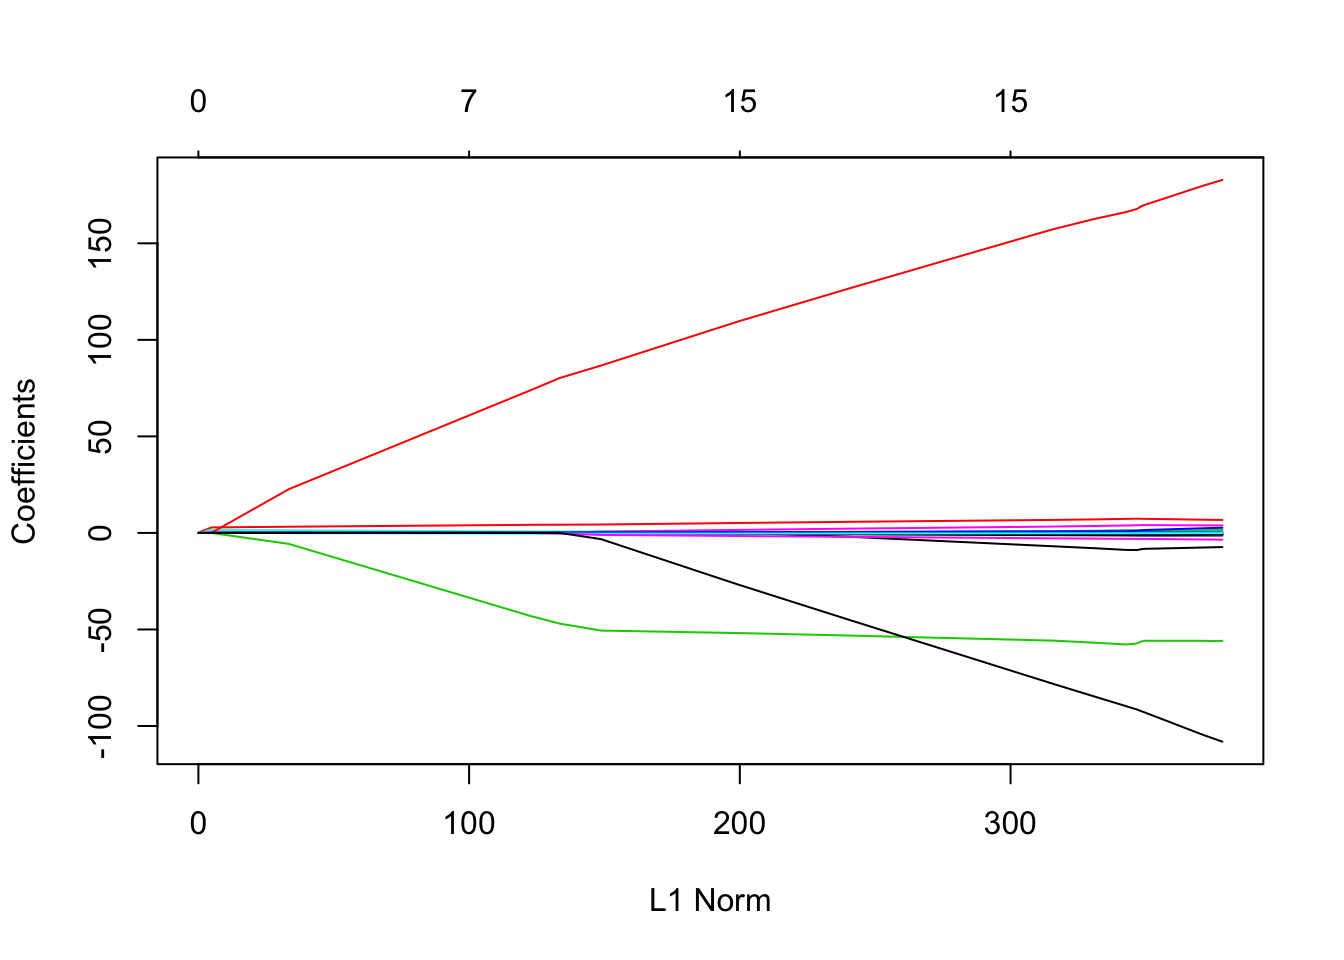
\includegraphics{bookdown-asmas_files/figure-latex/LassoModel-1.pdf}

Der Plot zeigt, wie sich der Strafterm für verschiedene Werte (durch
Farben codiert) verhält. Nun wollen wir den besten Wert für \(\lambda\)
bestimmen. Dies wird durch Kreuzvalidierung gemacht.

\begin{Shaded}
\begin{Highlighting}[]
\KeywordTok{set.seed} \NormalTok{(}\DecValTok{1}\NormalTok{)}
\NormalTok{cv.out <-}\StringTok{ }\KeywordTok{cv.glmnet} \NormalTok{(x[train ,],y[train],}\DataTypeTok{alpha =}\DecValTok{1}\NormalTok{)}
\NormalTok{bestlam <-}\StringTok{ }\NormalTok{cv.out$lambda.min}
\end{Highlighting}
\end{Shaded}

Der Anteil an Koeffizienten, welcher durch LASSO null gesetzt wird kann
mit folgenden Statements überprüft werden.

\begin{Shaded}
\begin{Highlighting}[]
\NormalTok{out <-}\StringTok{ }\KeywordTok{glmnet}\NormalTok{(x, y, }\DataTypeTok{alpha =} \DecValTok{1}\NormalTok{, }\DataTypeTok{lambda =} \NormalTok{grid)}
\NormalTok{lasso.coef <-}\StringTok{ }\KeywordTok{predict}\NormalTok{(out, }\DataTypeTok{type =} \StringTok{"coefficients"}\NormalTok{, }\DataTypeTok{s=}\NormalTok{bestlam )[}\DecValTok{1}\NormalTok{:}\DecValTok{20}\NormalTok{,]}
\NormalTok{lasso.coef}
\end{Highlighting}
\end{Shaded}

\begin{verbatim}
##   (Intercept)         AtBat          Hits         HmRun          Runs 
##  8.898370e-01 -5.575622e-03  2.007078e+00  0.000000e+00  0.000000e+00 
##           RBI         Walks         Years        CAtBat         CHits 
##  0.000000e+00  2.268641e+00 -3.428874e-02  0.000000e+00  0.000000e+00 
##        CHmRun         CRuns          CRBI        CWalks       LeagueN 
##  8.315024e-03  2.102106e-01  4.211554e-01  0.000000e+00  1.695962e+01 
##     DivisionW       PutOuts       Assists        Errors    NewLeagueN 
## -1.143553e+02  2.343374e-01  0.000000e+00 -6.607899e-01  0.000000e+00
\end{verbatim}

\chapter{Bayes'sche Ansätze}\label{bayessche-ansatze}

\section{Einführung}\label{einfuhrung}

In der Statistik gibt es zwei verschiedene Lehrmeinungen. Es sind dies

\begin{enumerate}
\def\labelenumi{\arabic{enumi}.}
\tightlist
\item
  die \textbf{Frequentisten} und
\item
  die \textbf{Bayesianer}.
\end{enumerate}

Alle bisher
\footnote{Hier ist nicht nur diese Vorlesung sondern auch die Züchtungslehre und die angewandet Zuchtwertschätzung gemeint}
vorgestellten statistischen Konzepte, so zum Beispiel
\texttt{Least\ Squares}, \texttt{Maximum\ Likelihood}, \texttt{REML} und
\texttt{BLUP} stammen aus dem Lager der Frequentisten.

Die Unterschiede zwischen Frequentisten und Bayesianern bestehen
hauptsächlich in

\begin{itemize}
\tightlist
\item
  deren Verständnis von Wahrscheinlichkeiten
\item
  deren Unterteilung von Modell- und Datenkomponenten
\item
  deren Techniken zur Schätzung von Parametern
\end{itemize}

Die folgende Tabelle gibt eine Übersicht über die Unterschiede.

\begin{tabular}{p{3cm}p{6cm}p{6cm}}
\hline
Was                            &  Frequentisten  &  Bayesianer \\
\hline
Wahrscheinlichkeiten           &  Eigenschaften von Zufallsvariablen, welche bei grossen Stichproben eintreten
                               &  Mass für Informationsgehalt unabhängig von Stichprobengrösse \\
Modell- und Datenkomponenten   &  Unterscheidung zwischen Modellparametern und Daten. Parameter sind unbekannt, Daten sind bekannt. Fehlende Daten werden ignoriert
                               &  Unterscheidung zwischen unbekannten und bekannten Grössen, unabhängig ob Parameter oder Daten. Fehlende Daten können simuliert werden \\
Schätztungen von Parametern    &  ML oder REML werden für Parameterschätzung verwendet
                               &  MCMC Zufallszahlen zur Approximation der gewünschten a posteriori Verteilungen \\
\hline
\end{tabular}

\section{Das Lineare Modell}\label{das-lineare-modell}

Die Bayes'sche Art der Parameterschätzung soll an einem einfachen
linearen Modell gezeigt werden. Angenommen, wir betrachten das Modell

\begin{equation}
y_i = \beta_0 + \beta_1 x_{i1} + \epsilon_i
\label{eq:BayLinMod}
\end{equation}

wobei \(y_i\) die \(i\)-te Beobachtung einer Zielgrösse ist, \(\beta_0\)
für den Achsenabschnitt steht, \(x_1\) eine erklärende Variable ist und
\(\epsilon_i\) für den Restterm steht. Für den Restterm nehmen wir an,
dass deren Varianz konstant gleich \(\sigma^2\) ist.

\subsection{Bekannte und Unbekannte}\label{bekannte-und-unbekannte}

Unter der Annahme, dass wir für die Zielgrösse \(y_i\) und die
erklärende Variable \(x_1\) keine fehlenden Daten haben, dann machen wir
als Bayesianer folgende Einteilung in bekannte und unbekannte Grössen.

und als \textbf{bekannte} Grössen

\begin{center}
\begin{tabular}{p{3cm}cc}
\hline
Was         &  bekannt  &  unbekannt \\
\hline
$y_i$       &    X      & \\
$x_1$       &    X      & \\
$\beta_0$   &           &      X \\
$\beta_1$   &           &      X \\
$\sigma^2$  &           &      X \\
\hline
\end{tabular}
\end{center}

\subsection{Vorgehen bei
Parameterschätzung}\label{vorgehen-bei-parameterschatzung}

Bayesianer basieren Schätzungen von unbekannten Grössen auf der
sogenannten \textbf{a posteriori Verteiung} der unbekannten Grössen
gegeben die bekannten Grössen. Die a posteriori Verteilung wird mithilfe
des \textbf{Satzes von Bayes} aufgrund der a priori Verteilung der
unbekannten und aufgrund der Likelihood berechnet.

Die Bezeichnungen ``a priori'' und ``a posteriori'' beziehen sich immer
auf den Zeitpunkt der Beobachtung der analysierten Daten. Die jeweiligen
Verteilungen quantifizieren den Informationsstand zu den Unbekannten um
jeweiligen Zeitpunkt. Dieses Konzept soll anhand der folgenden Grafik
verdeutlicht werden.

\begin{center}\includegraphics[width=8cm]{AprioriAposteriori} \end{center}

Für unser Beispiel des einfachen linearen Modells, definieren wir zuerst
den Vektor \(\mathbf{\beta}\) als

\[\beta = \left[\begin{array}{c} \beta_0  \\  \beta_1 \end{array} \right].\]

Die Beobachtungen \(y_i\) fassen wir ebenfalls zu einem Vektor \(y\)
zusammen. Für den Moment nehmen wir an, dass \(\sigma^2\) bekannt sei.
Eine Bayes'sche Parameterschätzung für \(\beta\) basiert dann auf der a
posteriori Verteilung \(f(\beta | y, \sigma^2)\) der Unbekannten
\(\beta\) gegeben die Bekannten \(y\) und \(\sigma^2\). Diese a
posteriori Verteilung lässt sich mit dem Satz von Bayes, wie folgt
berechnen

\begin{eqnarray}
f(\beta | y, \sigma^2) & =       & \frac{f(\beta, \sigma^2, y)}{f(y, \sigma^2)} \nonumber \\
                       & =       & \frac{f(y | \beta, \sigma^2)f(\beta)f(\sigma^2)}{f(y, \sigma^2)} \nonumber \\
                       & \propto & f(y | \beta, \sigma^2)f(\beta)f(\sigma^2)
\label{LinModAPostProb}
\end{eqnarray}

In Gleichung (\ref{LinModAPostProb}) konnten wir die a posteriori
Verteilung \(f(\beta | y, \sigma^2)\) als Produkt der a priori
Verteilungen (\(f(\beta)\) und \(f(\sigma^2)\)) der unbekannten Grössen
\(\beta\) und \(\sigma^2\) und der Likelihood \(f(y | \beta, \sigma^2)\)
ausdrücken. Der Faktor \(f(y, \sigma^2)^{-1}\) (Term im Nenner)
entspricht der sogenannten Normalisierungskonstanten und ist nicht
weiter von Interesse. Somit wird die a posteriori Verteilung oft als
Proporzionalitätsbeziehung angegeben.

Die a posteriori Verteilung \(f(\beta | y, \sigma^2)\) ist in vielen
Fällen nicht explizit darstellbar. Das war lange ein Problem, welches
die Anwendung von Bayes'schen Analysen sehr einschränkte. Zwei
Entwicklungen haben dieses Problem beseitigt.

\begin{enumerate}
\def\labelenumi{\arabic{enumi}.}
\tightlist
\item
  In seinem Paper (\citet{Besa1974}) zeigte Julian Besag, dass jede
  posteriori Verteilung durch eine Serie von Zufallszahlen aus den
  voll-bedingten Verteilungen bestimmt ist. Für unser Beispiel lauten
  die voll-bedingten Verteilungen: Bedingte Verteilung von \(\beta_0\)
  gegeben alle anderen Grössen: \(f(\beta_0 | \beta_1, \sigma^2, y)\),
  bedingte Verteilung von \(\beta_1\) gegeben alle anderen Grössen:
  \(f(\beta_1 | \beta_0, \sigma^2, y)\).
\item
  Die Entwicklung von effizienten Pseudo-Zufallszahlen-Generatoren auf
  dem Computer.
\end{enumerate}

\section{Gibbs Sampler}\label{gibbs-sampler}

Die Umsetzung der beiden oben aufgelisteten Punkte führt zu einer
Prozedur, welche als \textbf{Gibbs Sampler} bezeichnet wird. Wenden wir
den Gibbs Sampler auf einfaches lineares Regressionsmodell an, dann
resultiert das folgende Vorgehen bei der Analyse. Unabhängig vom
verwendeten Modell läuft die Konstruktion einer Gibbs Sampling Prozedur
immer in den folgenden Schritten ab. Diese Schritte können für die
meisten Analysen wie ein Kochbuchrezept verwendet werden.

\begin{enumerate}
\def\labelenumi{\arabic{enumi}.}
\tightlist
\item
  Bestimmung der a priori Verteilungen für die unbekannten Grössen.
\item
  Bestimmung der Likelihood
\item
  Bestimmung der voll-bedingten Verteilungen
\end{enumerate}

\subsection{A priori Verteilungen}\label{a-priori-verteilungen}

In unserem Bespiel handelt es sich dabei um \(f(\beta)\) und
\(f(\sigma^2)\). In den meisten Fällen, wenn man das erste Mal eine
bestimmte Art von Daten analysisern soll, empfielt es sich eine
sogenannte uniformative a priori Verteilung zu wählen. Eine
uninformative a priori Verteilung bedeutet einfach, dass deren
Dichtewert überall gleich, also eine Konstante ist. Wenden wir zum
Beispiel für die Unbekannte \(\beta\) eine uninformative a priori
Verteilung an, dann bedeutet das, dass wir \(f(\beta) = c\).

Alternativ zu der uniformativen a priori Verteilung gibt es auch a
priori Verteiungen für bestimmte unbekannte Grössen, welche als de-facto
Standard aktzeptiert sind. Ein Bespiel dafür ist die a priori Verteilung
der unbekannten Restvarianz, welche üblicherweise als
Inverse-Chi-Quadrat Verteilung angenommen wird.

\subsection{Likelihood}\label{likelihood}

Die Likelihood ist wie bei den Frequentisten als begingte Verteilung
(\(f(y | \beta, \sigma^2)\)) der Daten \(y\) gegeben die Parameter
(\(\beta\) und \(\sigma^2\)). Falls keine Daten fehlen, dann ist die
Bayes'sche Likelihood und die frequentistische Likelihood gleich.

\subsection{Vollbedingte Verteilungen}\label{vollbedingte-verteilungen}

Mit vollbedingten Verteilungen ist gemeint, dass für jede unbekannte
Grösse die bedingte Verteilung gegeben alle anderen Grössen bestimmt
wird. In unserem Bespiel des linearen Regressionsmodells haben wir zwei
unbekannte Grössen \(\beta_0\) und \(\beta_1\). Somit haben wir auch
zwei vollbedingte Verteilungen. Unter der Annahme, dass unsere Daten
(\(y\)) einer Normalverteilung folgen, resultieren die folgenden
vollbedingten Verteilungen.

\vspace{2ex}

\begin{center}
\begin{tabular}{lll}
\hline
unbekannte Grösse  &  unbekannte Grösse                    &  resultierende Verteilung \\
\hline
$\beta_0$          &  $f(\beta_0 | \beta_1, \sigma^2, y)$  &  $\mathcal{N}\left(\hat{\beta}_0, var(\hat{\beta}_0)\right)$ \\
$\beta_1$          &  $f(\beta_1 | \beta_0, \sigma^2, y)$  &  $\mathcal{N}\left(\hat{\beta}_1, var(\hat{\beta}_1)\right)$ \\
\hline
\end{tabular}
\end{center}

Aufgrund von Berechnungen, welche hier nicht gezeigt sind, können wir
die oben aufgelisteten vollbedingten Verteilungen bestimmen. Die
entsprechenden Verteilungen sind in der Kolonnen ganz rechts, welche mit
``resultierende Verteilung'' überschrieben ist, aufgelistet. Dabei steht
\(\mathcal{N}()\) für die Normalverteilung. Für die Erwartungswerte und
Varianzen wird das Modell in Gleichung (\ref{eq:BayLinMod}) leicht
umformuliert.

\begin{equation}
\mathbf{y} = \mathbf{1}\beta_0 + \mathbf{x}\beta_1 + \mathbf{\epsilon}
\label{eq:BayLinModReform}
\end{equation}

Aus dem obigen Modell bilden wir ein neues Modell, welches auf der
rechten Seite der Gleichung nur von \(\beta_0\) und
\(\mathbf{\epsilon}\) abhängt. Da wir wissen, dass die Verteilung der
Least Squares Schätzer eine Normalverteilung ist, werden wir diese für
die Bestimmung der vollbedingten Verteilungen verwenden.

\begin{equation}
\mathbf{w}_0 = \mathbf{1}\beta_0 + \mathbf{\epsilon}
\label{eq:BayLinModW0}
\end{equation}

wobei \(\mathbf{w}_0 = \mathbf{y} - \mathbf{x}\beta_1\). Aufgrund des
Modells in Gleichung (\ref{eq:BayLinModW0}) können wir den Least Squares
Schätzer für \(\beta_0\) aufstellen. Dieser lautet:

\begin{equation}
\hat{\beta}_0 = (\mathbf{1}^T\mathbf{1})^{-1}\mathbf{1}^T\mathbf{w}_0
\label{eq:Beta0LsEst}
\end{equation}

Die Varianz des Least Squares Schätzers für \(\beta_0\) lautet:

\begin{equation}
var(\hat{\beta}_0) = (\mathbf{1}^T\mathbf{1})^{-1}\sigma^2
\label{eq:VarBeta0LsEst}
\end{equation}

Analog zu \(\beta_0\) berechnen wir den Least Squares Schätzer für
\(\beta_1\) und dessen Varianz.

\begin{equation}
\hat{\beta}_1 = (\mathbf{x}^T\mathbf{x})^{-1}\mathbf{x}^T\mathbf{w}_1
\label{eq:Beta1LsEst}
\end{equation}

wobei \(\mathbf{w}_1 = \mathbf{y} - \mathbf{1}\beta_0\)

\begin{equation}
var(\hat{\beta}_1) = (\mathbf{x}^T\mathbf{x})^{-1}\sigma^2
\label{eq:VarBeta1LsEst}
\end{equation}

\subsection{Umsetzung des Gibbs
Samplers}\label{umsetzung-des-gibbs-samplers}

Der Gibbs Sampler wird durch wiederholtes ziehen von Zufallszahlen aus
den oben angegebenen vollbedingten Verteilungen umgesetzt. Das heisst,
wir setzen für alle unbekannten Grössen sinnvolle Startwerte ein. Für
\(\beta_0\) und \(\beta_1\) wählen wir \(0\) als Startwert. Dann
berechnen wir den Erwartungswert und die Varianz für die vollbedingte
Verteilung von \(\beta_0\). Aus dieser Verteilung ziehen wir einen neuen
Wert für \(\beta_0\). In einem zweiten Schritt berechnen wir den
Erwartungswert und die Varianz für die vollbedingte Verteilung von
\(\beta_1\), wobei wir für \(\beta_0\) schon den neuen Wert einsetzen.
Aus der Verteilung für \(\beta_1\) ziehen wir einen neuen Wert für
\(\beta_1\). Danach beginnen wir die Schritte wieder bei \(\beta_0\).
Diese Schrittabfolge wiederholen wir \(10000\) mal und speichern alle
gezogenen Werte für \(\beta_0\) und \(\beta_1\). Die Bayes'schen
Parameterschätzungen entsprechen dann den Mittelwerten der gespeicherten
Werte.

Der folgende R-Codeblock soll die Umsetzung des Gibbs Samplers für
\(\beta_0\) und \(\beta_1\) als Programm zeigen. Der Einfachheit halber
wurde \(\sigma^2\) konstant \(\sigma^2=1\) angenommen.

\begin{Shaded}
\begin{Highlighting}[]
\CommentTok{# ### Startwerte für beta0 und beta1}
\NormalTok{beta <– }\KeywordTok{c}\NormalTok{(}\DecValTok{0}\NormalTok{, }\DecValTok{0}\NormalTok{)}
\CommentTok{# ### Bestimmung der Anzahl Iterationen}
\NormalTok{niter <– }\DecValTok{10000}
\CommentTok{# ### Initialisierung des Vektors mit Resultaten}
\NormalTok{meanBeta <– }\KeywordTok{c}\NormalTok{(}\DecValTok{0}\NormalTok{, }\DecValTok{0}\NormalTok{)}
\NormalTok{for (iter in }\DecValTok{1}\NormalTok{:niter) \{}
  \CommentTok{# Ziehung des Wertes des Achsenabschnitts beta0}
  \NormalTok{w <– y -}\StringTok{ }\NormalTok{X[, }\DecValTok{2}\NormalTok{] *}\StringTok{ }\NormalTok{beta[}\DecValTok{2}\NormalTok{]}
  \NormalTok{x <– X[, }\DecValTok{1}\NormalTok{]}
  \NormalTok{xpxi <– }\DecValTok{1}\NormalTok{/(}\KeywordTok{t}\NormalTok{(x) %*%}\StringTok{ }\NormalTok{x)}
  \NormalTok{betaHat <– }\KeywordTok{t}\NormalTok{(x) %*%}\StringTok{ }\NormalTok{w *}\StringTok{ }\NormalTok{xpxi}
  \CommentTok{# ### neue Zufallszahl fuer beta0}
  \NormalTok{beta[}\DecValTok{1}\NormalTok{] <– }\KeywordTok{rnorm}\NormalTok{(}\DecValTok{1}\NormalTok{, betaHat, }\KeywordTok{sqrt}\NormalTok{(xpxi))}
  \CommentTok{# Ziehung der Steigung beta1}
  \NormalTok{w <– y -}\StringTok{ }\NormalTok{X[, }\DecValTok{1}\NormalTok{] *}\StringTok{ }\NormalTok{beta[}\DecValTok{1}\NormalTok{]}
  \NormalTok{x <– X[, }\DecValTok{2}\NormalTok{]}
  \NormalTok{xpxi <– }\DecValTok{1}\NormalTok{/(}\KeywordTok{t}\NormalTok{(x) %*%}\StringTok{ }\NormalTok{x)}
  \NormalTok{betaHat <– }\KeywordTok{t}\NormalTok{(x) %*%}\StringTok{ }\NormalTok{w *}\StringTok{ }\NormalTok{xpxi}
  \CommentTok{# ### neue Zufallszahl fuer beta1}
  \NormalTok{beta[}\DecValTok{2}\NormalTok{] <– }\KeywordTok{rnorm}\NormalTok{(}\DecValTok{1}\NormalTok{, betaHat, }\KeywordTok{sqrt}\NormalTok{(xpxi))}
  \NormalTok{meanBeta <– meanBeta +}\StringTok{ }\NormalTok{beta}
\NormalTok{\}}
\CommentTok{# ### Ausgabe der Ergebnisse}
\KeywordTok{cat}\NormalTok{(}\KeywordTok{sprintf}\NormalTok{(}\StringTok{"Achsenabschnitt = %6.3f }\CharTok{\textbackslash{}n}\StringTok{"}\NormalTok{, meanBeta[}\DecValTok{1}\NormalTok{]/iter))}
\KeywordTok{cat}\NormalTok{(}\KeywordTok{sprintf}\NormalTok{(}\StringTok{"Steigung = %6.3f }\CharTok{\textbackslash{}n}\StringTok{"}\NormalTok{, meanBeta[}\DecValTok{2}\NormalTok{]/iter))}
\end{Highlighting}
\end{Shaded}

\chapter*{Abkürzungen}\label{abkurzungen}
\addcontentsline{toc}{chapter}{Abkürzungen}

\begin{tabular}{l|l}
\hline
Abbreviation & Meaning\\
\hline
QTL & Quatitative Trait Loci\\
\hline
GWAS & Genome Wide Association Study\\
\hline
GLMM & Generalized Linear Mixed Models\\
\hline
i.i.d. & independent, identically distributed\\
\hline
QQ & Quantil Quantil\\
\hline
LASSO & Least Absolute Shrinkage And Selection Operator\\
\hline
REML & Restricted oder Residual Maximum Likelihood\\
\hline
ML & Maximum Likelihood\\
\hline
MCMC & Markov Chain Monte Carlo\\
\hline
\end{tabular}

\bibliography{ASMNW.bib}


\end{document}
